\chapter{Geometrija v ravnini}

\section{Osnovni geometrijski pojmi}

            
                Evklid je v prvi knjigi \textit{Elementov} postavil $23$ 'opredelitev' temeljnih geometrijskih pojmov.
                Med njimi so:
                \begin{itemize}
                    \item \textbf{Točka} je tisto, kar nima delov -- nima razsežnosti.
                    \item \textbf{Črta} je dolžina brez širine -- ena razsežnost.
                    \item \textbf{Ploskev} je tisto, kar ima samo dolžino in širino -- dve razsežnosti.
                \end{itemize}
            
                ~
            
                Tem trditvam sledijo \textbf{aksiomi} (temeljne resnice) -- privzamemo jih kot veljavne hipoteze,
                 \textbf{izreki}~-- dokazujemo jih z aksiomi in prej dokazanimi izreki, 
                 in \textbf{definicije} -- opisi novih pojmov in lastnosti.
            
        
                ~
        
            \subsection*{Incidenčni aksiomi}

            \begin{definicija}
                \textit{Incidenca} je relacija, ki povezuje točko in premico -- premica in točka sta v relaciji,
                 če točka leži na premici; $A~R~p$, če $A\in p$.
            \end{definicija}

            \begin{aksiom}
                Za dve različni točki $A$ in $B$ obstaja natanko določena premica $p$, tako da točki $A$ in $B$ ležita na njej.
            \end{aksiom}

            \begin{aksiom}
                Za vsako premico $p$ obstajata vsaj dve različni točki $P$ in $Q$, ki ležita na njej.
            \end{aksiom}

            \begin{aksiom}
                Obstajajo tri različne točke, ki ne ležijo hkrati na isti premici.
            \end{aksiom}
        

            ~
        
            \begin{definicija}
                Točke $A_1, A_2, A_3, \dots$, ki ležijo na isti premici, so \textbf{kolinearne}, 
                če ne ležijo na isti premici, pa so \textbf{nekolinearne}.
            \end{definicija}

            ~

            \begin{izrek}
                Dve različni premici imata lahko največ eno skupno točko.
            \end{izrek}

            \begin{definicija}
                Premici, ki imata natanko eno skupno točko, se \textbf{sekata}, imenujemo ju \textbf{sečnici},
                njuno skupno točko pa \textbf{presečišče} premic.
            \end{definicija}

            \begin{definicija}
                Premici, ki ležita na isti ravnini in nimata nobene skupne točke ali imata vse točke skupne -- sovpadata, sta \textbf{vzporedni}, imenujemo ju \textbf{vzporednici}.
            \end{definicija}
        

            ~
        
            \begin{aksiom}
                Če so tri različne točke kolinearne, ena vedno leži med drugima dvema.

                \begin{figure}[H]
                    \centering
                    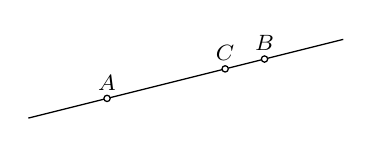
\begin{tikzpicture}
                        % \clip (0,0) rectangle (14.000000,10.000000);
                        {\footnotesize

                        % Drawing line A B
                        \draw [line width=0.016cm] (1.000000,1.250000) -- (1.961194,1.490299);%
                        \draw [line width=0.016cm] (2.038806,1.509701) -- (3.461194,1.865299);%
                        \draw [line width=0.016cm] (3.538806,1.884701) -- (3.961194,1.990299);%
                        \draw [line width=0.016cm] (4.038806,2.009701) -- (5.000000,2.250000);%

                        % Marking point A by circle
                        \draw [line width=0.016cm] (2.000000,1.500000) circle (0.040000);%
                        \draw (2.000000,1.500000) node [anchor=south] { $A$ };%

                        % Marking point C by circle
                        \draw [line width=0.016cm] (3.500000,1.875000) circle (0.040000);%
                        \draw (3.500000,1.875000) node [anchor=south] { $C$ };%

                        % Marking point B by circle
                        \draw [line width=0.016cm] (4.000000,2.000000) circle (0.040000);%
                        \draw (4.000000,2.000000) node [anchor=south] { $B$ };%
                        }
                    \end{tikzpicture}
                \end{figure}
            \end{aksiom}

            \begin{aksiom}
                Če sta $A$ in $B$ različni točki premice $p$, potem na premici $p$ ležita vsaj še točki $C$ in $D$,
                in sicer $C$ leži med $A$ in $B$, $D$ pa tako, da je $C$ med $A$ in $D$.

                \begin{figure}[H]
                    \centering
                    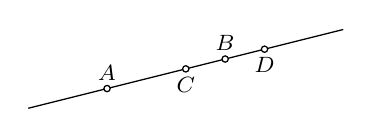
\begin{tikzpicture}
                        % \clip (0,0) rectangle (14.000000,10.000000);
                        {\footnotesize

                        % Drawing line A B
                        \draw [line width=0.016cm] (1.000000,1.250000) -- (1.961194,1.490299);%
                        \draw [line width=0.016cm] (2.038806,1.509701) -- (2.961194,1.740299);%
                        \draw [line width=0.016cm] (3.038806,1.759701) -- (3.461194,1.865299);%
                        \draw [line width=0.016cm] (3.538806,1.884701) -- (3.961194,1.990299);%
                        \draw [line width=0.016cm] (4.038806,2.009701) -- (5.000000,2.250000);%

                        % Marking point A by circle
                        \draw [line width=0.016cm] (2.000000,1.500000) circle (0.040000);%
                        \draw (2.000000,1.500000) node [anchor=south] { $A$ };%

                        % Marking point C by circle
                        \draw [line width=0.016cm] (3.000000,1.750000) circle (0.040000);%
                        \draw (3.000000,1.750000) node [anchor=north] { $C$ };%

                        % Marking point B by circle
                        \draw [line width=0.016cm] (3.500000,1.875000) circle (0.040000);%
                        \draw (3.500000,1.875000) node [anchor=south] { $B$ };%

                        % Marking point D by circle
                        \draw [line width=0.016cm] (4.000000,2.000000) circle (0.040000);%
                        \draw (4.000000,2.000000) node [anchor=north] { $D$ };%
                        }
                    \end{tikzpicture}
                \end{figure}
            \end{aksiom}

            \begin{izrek}
                Med dvema različnima točkama premice je neskončno mnogo točk.
            \end{izrek}

        
            ~

        
            \begin{definicija}
                Množica točk premice, ki ležijo med različnima točkama $A$ in $B$, vključno z $A$ in $B$,
                je \textbf{daljica~$AB$}. Točki $A$ in $B$ sta njeni \textbf{krajišči}.

                \begin{figure}[H]
                    \centering
                    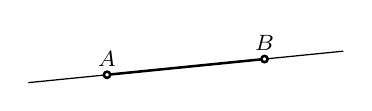
\begin{tikzpicture}
                        % \clip (0,0) rectangle (14.000000,10.000000);
                        {\footnotesize

                        % Drawing line A B
                        \draw [line width=0.016cm] (1.000000,1.400000) -- (1.960199,1.496020);%
                        \draw [line width=0.016cm] (2.039801,1.503980) -- (3.960199,1.696020);%
                        \draw [line width=0.016cm] (4.039801,1.703980) -- (5.000000,1.800000);%

                        % Drawing segment A B
                        \draw [line width=0.032cm] (2.039801,1.503980) -- (3.960199,1.696020);%

                        % Marking point A by circle
                        \draw [line width=0.032cm] (2.000000,1.500000) circle (0.040000);%
                        \draw (2.000000,1.500000) node [anchor=south] { $A$ };%

                        % Marking point B by circle
                        \draw [line width=0.032cm] (4.000000,1.700000) circle (0.040000);%
                        \draw (4.000000,1.700000) node [anchor=south] { $B$ };%
                        }
                    \end{tikzpicture}
                \end{figure}
            \end{definicija}

            \begin{definicija}
                Poljubna točka premice razdeli premico na dva \textbf{poltraka}. To točko imenujemo \textbf{izhodišče}, ponavadi jo označimo z $O$.

                \begin{figure}[H]
                    \centering
                    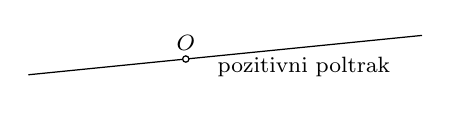
\begin{tikzpicture}
                        % \clip (0,0) rectangle (14.000000,10.000000);
                        {\footnotesize

                        % Drawing line O B
                        \draw [line width=0.016cm] (1.000000,1.300000) -- (2.960199,1.496020);%
                        \draw [line width=0.016cm] (3.039801,1.503980) -- (6.000000,1.800000);%

                        % Marking point O by circle
                        \draw [line width=0.016cm] (3.000000,1.500000) circle (0.040000);%
                        \draw (3.000000,1.500000) node [anchor=south] { $O$ };%

                        % Marking point poz
                        \draw (4.500000,1.400000) node  {pozitivni poltrak };%
                        }
                    \end{tikzpicture}
                \end{figure}
            \end{definicija}

            \begin{definicija}
                Premica, na kateri leži daljica oziroma poltrak, je \textbf{nosilka} daljice oziroma poltraka.
            \end{definicija}
        

            ~
        
            \begin{definicija}
                \textbf{Enostavni lik} je množica točk v ravnini, ki jo omejuje sklenjena krivulja, ki sama sebe ne seka.
            \end{definicija}

            \begin{definicija}

                Množica točk v ravnini je \textbf{konveksna}, če za poljubni točki $A$ in $B$ iz te množice velja, da je daljica $AB$ njena podmnožica.
                
                \begin{multicols}{2}
                $$ \mathcal{M}\text{~konveksna} \Leftrightarrow \forall A, B\in\mathcal{M}\Rightarrow AB\subseteq\mathcal{M} $$
                ~\\~

                \begin{figure}[H]
                    \centering
                    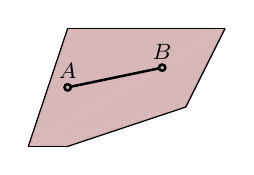
\begin{tikzpicture}
                        % \clip (0,0) rectangle (14.000000,10.000000);
                        {\footnotesize

                        % Changing color 215 183 183
                        \definecolor{r215g183b183}{rgb}{0.843137,0.717647,0.717647}%
                        \color{r215g183b183}% 

                        % Filling triangle C D E
                        \fill (1.500000,1.500000) -- (2.000000,1.500000) -- (3.500000,2.000000);%

                        % Filling triangle C E F
                        \fill (1.500000,1.500000) -- (3.500000,2.000000) -- (4.000000,3.000000);%

                        % Filling triangle C F G
                        \fill (1.500000,1.500000) -- (4.000000,3.000000) -- (2.000000,3.000000);%

                        % Changing color 0 0 0
                        \definecolor{r0g0b0}{rgb}{0.000000,0.000000,0.000000}%
                        \color{r0g0b0}% 

                        % Drawing segment C D
                        \draw [line width=0.016cm] (1.500000,1.500000) -- (2.000000,1.500000);%

                        % Drawing segment D E
                        \draw [line width=0.016cm] (2.000000,1.500000) -- (3.500000,2.000000);%

                        % Drawing segment E F
                        \draw [line width=0.016cm] (3.500000,2.000000) -- (4.000000,3.000000);%

                        % Drawing segment F G
                        \draw [line width=0.016cm] (4.000000,3.000000) -- (2.000000,3.000000);%

                        % Drawing segment G C
                        \draw [line width=0.016cm] (2.000000,3.000000) -- (1.500000,1.500000);%

                        % Marking point A by circle
                        \draw [line width=0.032cm] (2.000000,2.250000) circle (0.040000);%
                        \draw (2.000000,2.250000) node [anchor=south] { $A$ };%

                        % Marking point B by circle
                        \draw [line width=0.032cm] (3.200000,2.500000) circle (0.040000);%
                        \draw (3.200000,2.500000) node [anchor=south] { $B$ };%

                        % Drawing segment A B
                        \draw [line width=0.032cm] (2.039159,2.258158) -- (3.160841,2.491842);%
                        \color{black}
                        }
                    \end{tikzpicture}
                \end{figure}
                
            \end{multicols}

                Množica točk, ki ni konveksna, je \textbf{nekonveksna} oziroma \textbf{konkavna}.
                
            \begin{multicols}{2}
                
                $$ \mathcal{M}\text{~nekonveksna} \Leftrightarrow \exists A, B\in\mathcal{M}\Rightarrow AB\not\subset\mathcal{M} $$
                ~\\~

                \begin{figure}[H]
                    \centering
                    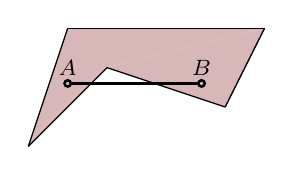
\begin{tikzpicture}
                        % \clip (0,0) rectangle (14.000000,10.000000);
                        {\footnotesize

                        % Changing color 215 183 183
                        \definecolor{r215g183b183}{rgb}{0.843137,0.717647,0.717647}%
                        \color{r215g183b183}% 

                        % Filling triangle C D G
                        \fill (1.500000,1.500000) -- (2.500000,2.500000) -- (2.000000,3.000000);%

                        % Filling triangle D E F
                        \fill (2.500000,2.500000) -- (4.000000,2.000000) -- (4.500000,3.000000);%

                        % Filling triangle D F G
                        \fill (2.500000,2.500000) -- (4.500000,3.000000) -- (2.000000,3.000000);%

                        % Changing color 0 0 0
                        \definecolor{r0g0b0}{rgb}{0.000000,0.000000,0.000000}%
                        \color{r0g0b0}% 

                        % Drawing segment C D
                        \draw [line width=0.016cm] (1.500000,1.500000) -- (2.500000,2.500000);%

                        % Drawing segment D E
                        \draw [line width=0.016cm] (2.500000,2.500000) -- (4.000000,2.000000);%

                        % Drawing segment E F
                        \draw [line width=0.016cm] (4.000000,2.000000) -- (4.500000,3.000000);%

                        % Drawing segment F G
                        \draw [line width=0.016cm] (4.500000,3.000000) -- (2.000000,3.000000);%

                        % Drawing segment G C
                        \draw [line width=0.016cm] (2.000000,3.000000) -- (1.500000,1.500000);%

                        % Marking point A by circle
                        \draw [line width=0.032cm] (2.000000,2.300000) circle (0.040000);%
                        \draw (2.000000,2.300000) node [anchor=south] { $A$ };%

                        % Marking point B by circle
                        \draw [line width=0.032cm] (3.700000,2.300000) circle (0.040000);%
                        \draw (3.700000,2.300000) node [anchor=south] { $B$ };%

                        % Drawing segment A B
                        \draw [line width=0.032cm] (2.040000,2.300000) -- (3.660000,2.300000);%
                        \color{black}
                        }
                    \end{tikzpicture}
                \end{figure}
            \end{multicols}   

        \end{definicija}
        

        ~
        
            \begin{definicija}
                Dva poltraka s skupnim izhodiščem določata dva \textbf{kota}.
                Izhodišče poltrakov imenujemo \textbf{vrh} kota, poltraka pa imenujemo \textbf{kraka} kota.
                
                \begin{figure}[H]
                    \centering
                    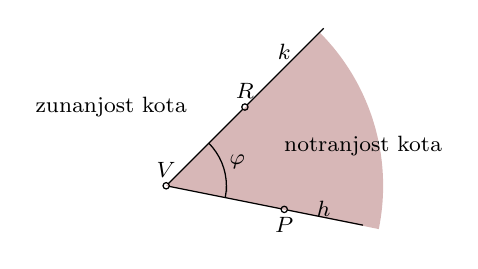
\begin{tikzpicture}
                        % \clip (0,0) rectangle (14.000000,10.000000);
                        {\footnotesize

                        % Changing color 215 183 183
                        \definecolor{r215g183b183}{rgb}{0.843137,0.717647,0.717647}%
                        \color{r215g183b183}% 

                        % Filling circle arc V B 56.31
                        \fill (2.500000,2.500000) -- (5.200000,1.949999) -- (5.204824,1.974235) arc (349:360:2.755449 and 2.755449) --(5.255449,2.500000) arc (0:44:2.755449 and 2.755449) -- (4.455318,4.441451) -- cycle;%

                        % Changing color 0 0 0
                        \definecolor{r0g0b0}{rgb}{0.000000,0.000000,0.000000}%
                        \color{r0g0b0}% 

                        % Drawing line V P
                        % \draw [line width=0.016cm] (1.000000,2.800000) -- (2.460777,2.507845);%
                        \draw [line width=0.016cm] (2.539223,2.492155) -- (3.960777,2.207845);%
                        \draw [line width=0.016cm] (4.039223,2.192155) -- (5.000000,2.000000);%

                        % Drawing line V R
                        % \draw [line width=0.016cm] (1.000000,1.000000) -- (2.471716,2.471716);%
                        \draw [line width=0.016cm] (2.528284,2.528284) -- (3.471716,3.471716);%
                        \draw [line width=0.016cm] (3.528284,3.528284) -- (4.500000,4.500000);%

                        % Marking point V by circle
                        \draw [line width=0.016cm] (2.500000,2.500000) circle (0.040000);%
                        \draw (2.500000,2.500000) node [anchor=south] { $V$ };%

                        % Marking point P by circle
                        \draw [line width=0.016cm] (4.000000,2.200000) circle (0.040000);%
                        \draw (4.000000,2.200000) node [anchor=north] { $P$ };%

                        % Marking point R by circle
                        \draw [line width=0.016cm] (3.500000,3.500000) circle (0.040000);%
                        \draw (3.500000,3.500000) node [anchor=south] { $R$ };%

                        % Marking point h
                        \draw (4.500000,2.000000) node [anchor=south] { $h$ };%

                        % Marking point k
                        \draw (4.000000,4.000000) node [anchor=south] { $k$ };%

                        % Drawing arc V A 56.31
                        \draw [line width=0.016cm] (3.250000,2.350000) -- (3.250800,2.354059) arc (349:360:0.764853 and 0.764853) --(3.264853,2.500000) arc (0:45:0.764853 and 0.764853);%

                        % Marking point \varphi
                        \draw (3.200000,2.800000) node [anchor=west] { $\varphi$ };%

                        % Marking point zun
                        \draw (1.800000,3.500000) node  { zunanjost kota };%

                        % Marking point not
                        \draw (5.000000,3.000000) node  { notranjost kota };%
                        \color{black}
                        }
                    \end{tikzpicture}
                \end{figure}
            \end{definicija}

            
                Če poltraka ne ležita na isti premici, je eden od kotov konveksen, drugi pa je nekonveksen.
            

            
                Kot lahko označimo na več načinov:
                \begin{itemize}
                    \item $\angle(h,k)$, kjer sta $h$ in $k$ poltraka, ki kot določata;
                    \item $\angle PVR$, kjer je $P$ točka na enem poltraku, $V$ vrh kota in $R$ točka na drugem poltraku;
                    \item $\alpha, \beta, \gamma, \dots$ -- z grškimi črkami.
                \end{itemize}
            
        
                ~

        
            \begin{definicija}
                Če poltraka s skupnim izhodiščem ležita na isti premici, vendar na različnih straneh izhodišča,
                določata dva enaka konveksna kota -- \textbf{iztegnjena kota}.

                \begin{figure}[H]
                    \centering
                    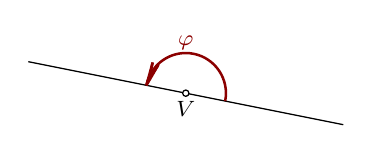
\begin{tikzpicture}
                        % \clip (0,0) rectangle (14.000000,10.000000);
                        {\footnotesize

                        % Drawing line V h
                        \draw [line width=0.016cm] (1.000000,2.000000) -- (2.960777,1.607845);%
                        \draw [line width=0.016cm] (3.039223,1.592155) -- (5.000000,1.200000);%

                        % Marking point V by circle
                        \draw [line width=0.016cm] (3.000000,1.600000) circle (0.040000);%
                        \draw (3.000000,1.600000) node [anchor=north] { $V$ };%

                        % Changing color 139 0 0
                        \definecolor{r139g0b0}{rgb}{0.545098,0.000000,0.000000}%
                        \color{r139g0b0}% 

                        % Drawing arc V h 180.00
                        \draw [line width=0.032cm] (3.500000,1.500000) -- (3.500534,1.502706) arc (349:360:0.509902 and 0.509902) --(3.509902,1.600000) arc (0:168:0.509902 and 0.509902) -- (2.500000,1.700000);%

                        % Marking point \varphi
                        \draw (3.000000,2.050000) node [anchor=south] { $\varphi$ };%

                        % Drawing arrow C A 1.00
                        \draw [line width=0.032cm] (2.651137,1.959148) -- (2.500000,1.700000);%
                        \draw [line width=0.032cm] (2.651137,1.959148) -- (2.538342,1.791430);%
                        \draw [line width=0.032cm] (2.578914,1.989435) -- (2.500000,1.700000);%
                        \draw [line width=0.032cm] (2.578914,1.989435) -- (2.538342,1.791430);%
                        \color{black}
                        }
                    \end{tikzpicture}
                \end{figure}
            \end{definicija}

            \begin{definicija}
                Če se poltraka na isti premici prekrivata, določata \textbf{polni kot} ali \textbf{ničelni kot}.

                \begin{figure}[H]
                    \centering
                    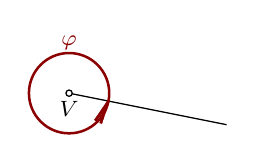
\begin{tikzpicture}
                        % \clip (0,0) rectangle (14.000000,10.000000);
                        {\footnotesize

                        % Drawing line V h
                        % \draw [line width=0.016cm] (1.000000,2.000000) -- (2.960777,1.607845);%
                        \draw [line width=0.016cm] (3.039223,1.592155) -- (5.000000,1.200000);%

                        % Marking point V by circle
                        \draw [line width=0.016cm] (3.000000,1.600000) circle (0.040000);%
                        \draw (3.000000,1.600000) node [anchor=north] { $V$ };%

                        % Changing color 139 0 0
                        \definecolor{r139g0b0}{rgb}{0.545098,0.000000,0.000000}%
                        \color{r139g0b0}% 

                        % Drawing arc V h 360.00
                        \draw [line width=0.032cm] (3.000000,1.600000) circle (0.509902);%

                        % Marking point \varphi
                        \draw (3.000000,2.050000) node [anchor=south] { $\varphi$ };%

                        % Drawing arrow k h 1.00
                        \draw [line width=0.032cm] (3.331960,1.251479) -- (3.500000,1.500000);%
                        \draw [line width=0.032cm] (3.331960,1.251479) -- (3.455661,1.411322);%
                        \draw [line width=0.032cm] (3.402008,1.216456) -- (3.500000,1.500000);%
                        \draw [line width=0.032cm] (3.402008,1.216456) -- (3.455661,1.411322);%
                        \color{black}
                        }
                    \end{tikzpicture} ~~~~~
                    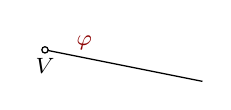
\begin{tikzpicture}
                        % \clip (0,0) rectangle (14.000000,10.000000);
                        {\footnotesize

                        % Drawing line V h
                        % \draw [line width=0.016cm] (1.000000,2.000000) -- (2.960777,1.607845);%
                        \draw [line width=0.016cm] (3.039223,1.592155) -- (5.000000,1.200000);%

                        % Marking point V by circle
                        \draw [line width=0.016cm] (3.000000,1.600000) circle (0.040000);%
                        \draw (3.000000,1.600000) node [anchor=north] { $V$ };%

                        % Changing color 139 0 0
                        \definecolor{r139g0b0}{rgb}{0.545098,0.000000,0.000000}%
                        \color{r139g0b0}% 

                        % Marking point \varphi
                        \draw (3.500000,1.500000) node [anchor=south] { $\varphi$ };%
                        \color{black}
                        }
                    \end{tikzpicture}
                \end{figure}

            \end{definicija}
        
            ~

        
            \begin{definicija}
                Kota s skupnim vrhom, ki imata en skupen krak, presek njunih notranjosti pa je prazen, sta \textbf{sosedna kota}.

                \begin{figure}[H]
                    \centering
                    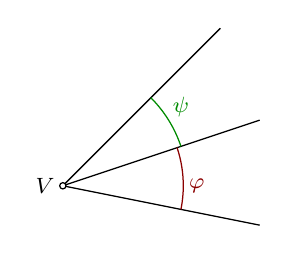
\begin{tikzpicture}
                        % \clip (0,0) rectangle (14.000000,10.000000);
                        {\footnotesize

                        % Drawing line V P
                        \draw [line width=0.016cm] (4.000000,1.000000) -- (1.539223,1.492155);%
                        % \draw [line width=0.016cm] (1.460777,1.507845) -- (1.000000,1.600000);%

                        % Drawing line V Q
                        % \draw [line width=0.016cm] (1.000000,1.333333) -- (1.462053,1.487351);%
                        \draw [line width=0.016cm] (1.537947,1.512649) -- (4.000000,2.333333);%

                        % Drawing line V R
                        % \draw [line width=0.016cm] (1.000000,1.000000) -- (1.471716,1.471716);%
                        \draw [line width=0.016cm] (1.528284,1.528284) -- (3.500000,3.500000);%

                        % Marking point V by circle
                        \draw [line width=0.016cm] (1.500000,1.500000) circle (0.040000);%
                        \draw (1.500000,1.500000) node [anchor=east] { $V$ };%

                        % Changing color 139 0 0
                        \definecolor{r139g0b0}{rgb}{0.545098,0.000000,0.000000}%
                        \color{r139g0b0}% 

                        % Drawing arc V P 29.74
                        \draw [line width=0.016cm] (3.000000,1.200000) -- (3.001601,1.208118) arc (349:360:1.529706 and 1.529706) --(3.029706,1.500000) arc (0:18:1.529706 and 1.529706) -- (2.951206,1.983735);%

                        % Marking point \varphi
                        \draw (3.200000,1.500000) node  { $\varphi$ };%

                        % Changing color 0 139 0
                        \definecolor{r0g139b0}{rgb}{0.000000,0.545098,0.000000}%
                        \color{r0g139b0}% 

                        % Drawing arc V Q 26.57
                        \draw [line width=0.016cm] (3.000000,2.000000) -- (2.994996,2.014768) arc (19:45:1.581139 and 1.581139);%

                        % Marking point \psi
                        \draw (3.000000,2.500000) node  { $\psi$ };%
                        \color{black}
                        }
                    \end{tikzpicture}
                \end{figure}
            \end{definicija}

            \begin{definicija}
                Sosedna kota, katerih kraka, ki  nista skupna, ležita na isti premici, sta \textbf{sokota}.
                
                \begin{figure}[H]
                    \centering
                    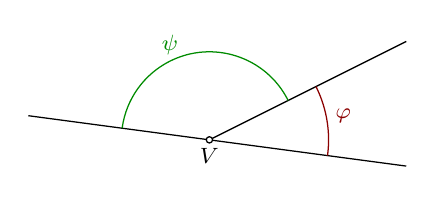
\begin{tikzpicture}
                        % \clip (0,0) rectangle (14.000000,10.000000);
                        {\footnotesize

                        % Drawing line V P
                        \draw [line width=0.016cm] (1.200000,1.806667) -- (3.460351,1.505287);%
                        \draw [line width=0.016cm] (3.539649,1.494713) -- (6.000000,1.166667);%

                        % Drawing line V Q
                        % \draw [line width=0.016cm] (2.700000,1.100000) -- (3.464223,1.482111);%
                        \draw [line width=0.016cm] (3.535777,1.517889) -- (6.000000,2.750000);%

                        % Marking point V by circle
                        \draw [line width=0.016cm] (3.500000,1.500000) circle (0.040000);%
                        \draw (3.500000,1.500000) node [anchor=north] { $V$ };%

                        % Changing color 139 0 0
                        \definecolor{r139g0b0}{rgb}{0.545098,0.000000,0.000000}%
                        \color{r139g0b0}% 

                        % Drawing arc V P 34.16
                        \draw [line width=0.016cm] (5.000000,1.300000) -- (5.001995,1.315578) arc (353:360:1.513275 and 1.513275) --(5.013275,1.500000) arc (0:26:1.513275 and 1.513275) -- (4.853514,2.176757);%

                        % Marking point \varphi
                        \draw (5.200000,1.800000) node  { $\varphi$ };%

                        % Changing color 0 139 0
                        \definecolor{r0g139b0}{rgb}{0.000000,0.545098,0.000000}%
                        \color{r0g139b0}% 

                        % Drawing arc V Q 145.84
                        \draw [line width=0.016cm] (4.500000,2.000000) -- (4.496176,2.007577) arc (27:172:1.118034 and 1.118034) -- (2.391774,1.647764);%

                        % Marking point \psi
                        \draw (3.000000,2.700000) node  { $\psi$ };%
                        \color{black}
                        }
                    \end{tikzpicture}
                \end{figure}
            \end{definicija}

        

            ~\\
        
            \begin{definicija}
                Tri nekolinearne točke $A$, $B$ in $C$ določajo \textbf{trikotnik} $\triangle ABC$.
                Točke $A$, $B$ in $C$ so \textbf{oglišča} trikotnika, daljice $AB$, $BC$ in $AC$ so njegove \textbf{stranice}.

            \begin{figure}[H]
                \centering
                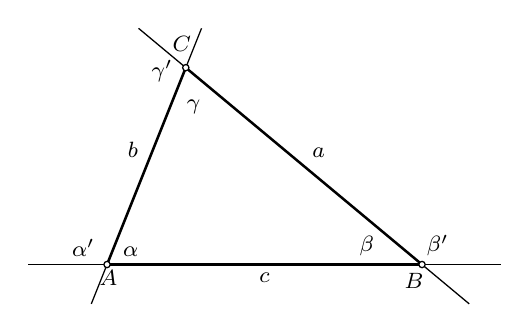
\begin{tikzpicture}
                    % \clip (0,0) rectangle (14.000000,10.000000);
                    {\footnotesize
                    
                    % Marking point A by circle
                    \draw [line width=0.016cm] (2.000000,1.500000) circle (0.040000);%
                    \draw (1.800000,1.530000) node [anchor=north west] { $A$ };%
                    
                    % Marking point B by circle
                    \draw [line width=0.016cm] (6.000000,1.500000) circle (0.040000);%
                    \draw (5.900000,1.500000) node [anchor=north] { $B$ };%
                    
                    % Marking point C by circle
                    \draw [line width=0.016cm] (3.000000,4.000000) circle (0.040000);%
                    \draw (2.950000,4.100000) node [anchor=south] { $C$ };%
                    
                    % Drawing line A B
                    \draw [line width=0.016cm] (1.000000,1.500000) -- (1.960000,1.500000);%
                    \draw [line width=0.016cm] (2.040000,1.500000) -- (5.960000,1.500000);%
                    \draw [line width=0.016cm] (6.040000,1.500000) -- (7.000000,1.500000);%
                    
                    % Drawing line B C
                    \draw [line width=0.016cm] (6.600000,1.000000) -- (6.030729,1.474393);%
                    \draw [line width=0.016cm] (5.969271,1.525607) -- (3.030729,3.974393);%
                    \draw [line width=0.016cm] (2.969271,4.025607) -- (2.400000,4.500000);%
                    
                    % Drawing line A C
                    \draw [line width=0.016cm] (1.800000,1.000000) -- (1.985144,1.462861);%
                    \draw [line width=0.016cm] (2.014856,1.537139) -- (2.985144,3.962861);%
                    \draw [line width=0.016cm] (3.014856,4.037139) -- (3.200000,4.500000);%
                    
                    % Marking point c
                    \draw (4.000000,1.500000) node [anchor=north] { $c$ };%
                    
                    % Marking point a
                    \draw (4.500000,2.750000) node [anchor=south west] { $a$ };%
                    
                    % Marking point b
                    \draw (2.500000,2.750000) node [anchor=south east] { $b$ };%
                    
                    % Marking point \gamma
                    \draw (3.100000,3.700000) node [anchor=north] { $\gamma$ };%
                    
                    % Marking point \gamma'
                    \draw (2.700000,4.200000) node [anchor=north] { $\gamma'$ };%
                    
                    % Marking point \beta
                    \draw (5.300000,1.500000) node [anchor=south] { $\beta$ };%
                    
                    % Marking point \beta'
                    \draw (6.200000,1.500000) node [anchor=south] { $\beta'$ };%
                    
                    % Marking point \alpha
                    \draw (2.300000,1.500000) node [anchor=south] { $\alpha$ };%
                    
                    % Marking point \alpha'
                    \draw (1.700000,1.500000) node [anchor=south] { $\alpha'$ };%
                    
                    % Drawing segment A B
                    \draw [line width=0.032cm] (2.040000,1.500000) -- (5.960000,1.500000);%
                    
                    % Drawing segment B C
                    \draw [line width=0.032cm] (5.969271,1.525607) -- (3.030729,3.974393);%
                    
                    % Drawing segment A C
                    \draw [line width=0.032cm] (2.014856,1.537139) -- (2.985144,3.962861);%
                    }
                \end{tikzpicture}
            \end{figure}

                Koti $\alpha$, $\beta$ in $\gamma$ so \textbf{notranji koti}, 
                njihovi sokoti $\alpha'$, $\beta'$ in $\gamma'$ pa so \textbf{zunanji koti} trikotnika.

            \end{definicija}

            
                Trikotnik je \textbf{pozitivno orientiran}, če si njegova oglišča sledijo v nasprotni smeri vrtenja urnega kazalca; 
                če si sledijo v smeri vrtenja urnega kazalca, pa je \textbf{negativno orientiran}.
            
        
            ~

        
            \begin{definicija}
                Točke $A_1, A_2, A_3, \dots, A_n$ v ravnini, od katerih nobene zaporedne tri niso kolinearne, določajo \textbf{$n$-kotnik}.
                Točke $A_1, A_2, A_3, \dots, A_n$ so \textbf{oglišča} $n$-kotnika;
                daljice, ki povezujejo sosedni oglišči, $A_1A_2, A_2A_3, \dots, A_nA_1$ so \textbf{stranice} $n$-kotnika;
                daljice, ki povezujejo po dve nesosedni oglišči, pa so \textbf{diagonale} $n$-kotnika.
            \end{definicija}

            
                Poljuben $n$-kotnika ima $$\dfrac{n(n-3)}{2}$$ diagonal -- iz vsakega od $n$ oglišč gre $n-3$ diagonal, vsaka pa je šteta dvakrat.
            
            ~
            
                Če za vsako nosilko stranice $n$-kotnika velja, da preostala oglišča ležijo na isti strani te nosilke, je $n$-kotnik \textbf{konveksen}.
            
        




        %%%%% naloge

        ~\\~\\

            \begin{naloga}
                Izračunajte število diagonal: $17$-kotnika, $31$-kotnika in $28$-kotnika.                
            \end{naloga}

            \begin{naloga}
                Ugotovite, ali obstaja $n$-kotnik, ki ima desetino toliko diagonal kot $28$-kotnik.
                Če obstaja, izračunajte, koliko stranic ima.
            \end{naloga}   
            
            \begin{naloga}
                Kateri $n$-kotnik ima štirikrat toliko diagonal kot stranic?
            \end{naloga}
        
            \begin{naloga}
                Izračunajte, kateri $n$-kotnik ima: $104$ diagonale, $230$ diagonal, $2n-5$ diagonal.
            \end{naloga}

            \begin{naloga}
                Pokažite, da ne obstaja $n$-kotnik, ki ima $13$ diagonal.  
            \end{naloga}
            

            \begin{naloga}
                Za vsako od spodnjih izjav ugotovite, ali je pravilna ali nepravilna.
                \begin{itemize}
                    \item Tri različne točke, so vedno nekolinearne.
                    \item Petkotnik ima enako število diagonal in stranic.
                    \item Štiri različne premice se sekajo v največ $4$ različnih točkah.
                    \item Skozi štiri kolinearne točke gredo tri različne premice.
                    \item Vzporedni premici imata lahko neskončno mnogo skupnih točk.
                \end{itemize}
            \end{naloga}

            \begin{naloga}
                Pokažite, da je število diagonal $25$-kotnika večkratnik števila njegovih stranic.
            \end{naloga}

            \begin{naloga}
                Vsota števila stranic in diagonal $n$-kotnika je $105$? Kateri $n$-kotnik je to?
            \end{naloga}
        

            \begin{naloga}
                Izračunajte, kateri $n$-kotnik ima toliko diagonal kot stranic.
            \end{naloga}

            \begin{naloga}
                Člani filatelističnega društva so se domenili, da si bodo za praznike spet pošiljali voščilnice po klasični pošti.
                Ko so se dobili po novem letu, so prinesli vse voščilnice in jih našteli $132$.
                Izračunajte, koliko članov društva, si je medseboj poslalo voščilnice.                
            \end{naloga}


        

\newpage
%%%%%%%%%%%%%%%%%%%%%%%%%%%%%%%%%%%%%%%


\section{Skladnost in merjenje}


    \begin{definicija}
        Dva lika $L$ in $L'$ sta \textbf{skladna}, če lahko lik $L$ prenesemo na lik $L'$ tako,
        da se popolnoma prekrijeta.

        Znak za skladnost je $\cong$.
    \end{definicija}

    
        \textbf{Skladnost} je v množici ravninskih likov \textit{ekvivalenčna relacija}, saj je:
        \begin{itemize}
            \item \textit{refleksivna}: $L\cong L$ -- vsaka množica je skladna sama s seboj;
            \item \textit{simetrična}: $L\cong L' \Rightarrow L'\cong L$ -- če je prva množica skladna z drugo, je tudi druga skladna s prvo;
            \item \textit{tranzitivna}: $L\cong L' \land L'\cong L'' \rightarrow L\cong L''$ -- če je prva množica skladna z drugo in druga skladna s tretjo, 
                    je tudi prva množica skladna s tretjo množico.
        \end{itemize}
    

~


    \begin{definicija}
        Kot, ki je skladen s svojim sokotom, je \textbf{pravi kot}.

        \begin{figure}[H]
            \centering
            \begin{tikzpicture}
            % \clip (0,0) rectangle (14.000000,10.000000);
            {\footnotesize

            % Drawing line V A
            \draw [line width=0.016cm] (1.000000,1.500000) -- (2.960000,1.500000);%
            \draw [line width=0.016cm] (3.040000,1.500000) -- (5.000000,1.500000);%

            % Drawing line V B
            % \draw [line width=0.016cm] (3.000000,1.000000) -- (3.000000,1.460000);%
            \draw [line width=0.016cm] (3.000000,1.540000) -- (3.000000,3.500000);%

            % Marking point V by circle
            \draw [line width=0.016cm] (3.000000,1.500000) circle (0.040000);%

            % Changing color 139 0 0
            \definecolor{r139g0b0}{rgb}{0.545098,0.000000,0.000000}%
            \color{r139g0b0}% 

            % Drawing arc V A 90.00
            \draw [line width=0.032cm] (3.800000,1.500000) arc (360:360:0.800000 and 0.800000) --(3.800000,1.500000) arc (0:90:0.800000 and 0.800000);%

            % Changing color 0 139 0
            \definecolor{r0g139b0}{rgb}{0.000000,0.545098,0.000000}%
            \color{r0g139b0}% 

            % Drawing arc V B 90.00
            \draw [line width=0.032cm] (3.000000,2.200000) arc (90:180:0.700000 and 0.700000);%
            \color{black}
            }
            \end{tikzpicture}

        \end{figure}
        
    \end{definicija}

    
        Če si kraka sledita v nasprotni smeri vrtenja urnega kazalca, je \textbf{orientacija kota pozitivna}, 
        če pa si sledita v smeri vrtenja urnega kazalca, pa je \textbf{orientacija kota negativna}.

        \begin{figure}[H]
                \centering
            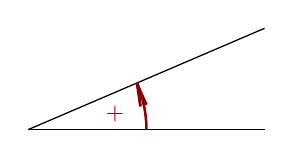
\begin{tikzpicture}
            % \clip (0,0) rectangle (14.000000,10.000000);
            {\footnotesize

            % Drawing segment A b
            \draw [line width=0.016cm] (1.500000,1.500000) -- (4.500000,1.500000);%

            % Drawing segment A C
            \draw [line width=0.016cm] (1.500000,1.500000) -- (4.500000,2.785714);%

            % Changing color 139 0 0
            \definecolor{r139g0b0}{rgb}{0.545098,0.000000,0.000000}%
            \color{r139g0b0}% 

            % Drawing arc A B 23.20
            \draw [line width=0.032cm] (3.000000,1.500000) arc (360:360:1.500000 and 1.500000) --(3.000000,1.500000) arc (0:23:1.500000 and 1.500000) -- (2.878718,2.090879);%

            % Drawing arrow Bb U 1.00
            \draw [line width=0.032cm] (2.923918,1.794304) -- (2.878718,2.090879);%
            \draw [line width=0.032cm] (2.923918,1.794304) -- (2.906321,1.995655);%
            \draw [line width=0.032cm] (2.999137,1.816108) -- (2.878718,2.090879);%
            \draw [line width=0.032cm] (2.999137,1.816108) -- (2.906321,1.995655);%

            % Marking point +
            \draw (2.600000,1.700000) node  { $+$ };%
            \color{black}
            }
            \end{tikzpicture} ~~~~~
            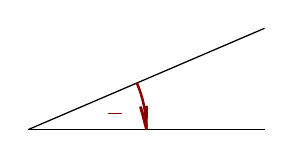
\begin{tikzpicture}
            % \clip (0,0) rectangle (14.000000,10.000000);
            {\footnotesize

            % Drawing segment A b
            \draw [line width=0.016cm] (1.500000,1.500000) -- (4.500000,1.500000);%

            % Drawing segment A C
            \draw [line width=0.016cm] (1.500000,1.500000) -- (4.500000,2.785714);%

            % Changing color 139 0 0
            \definecolor{r139g0b0}{rgb}{0.545098,0.000000,0.000000}%
            \color{r139g0b0}% 

            % Drawing arc A B 23.20
            \draw [line width=0.032cm] (3.000000,1.500000) arc (360:360:1.500000 and 1.500000) --(3.000000,1.500000) arc (0:23:1.500000 and 1.500000) -- (2.878718,2.090879);%

            % Drawing arrow Bb B 1.00
            \draw [line width=0.032cm] (3.001963,1.799994) -- (3.000000,1.500000);%
            \draw [line width=0.032cm] (3.001963,1.799994) -- (2.987703,1.598379);%
            \draw [line width=0.032cm] (2.924252,1.790280) -- (3.000000,1.500000);%
            \draw [line width=0.032cm] (2.924252,1.790280) -- (2.987703,1.598379);%

            % Marking point -
            \draw (2.600000,1.700000) node  { $-$ };%
            \color{black}
            }
            \end{tikzpicture}
        \end{figure}
    




        ~

    
        Daljici $AB$ in $CD$, ki nista skladni, lahko premaknemo na poljubni premici tako,
        da levi krajišči sovpadata in da eno od desnih krajišč, npr. $D$ leži med $A$ in $B$.
        V tem primeru je daljica $AB$ \textbf{daljša} od daljice $CD$ oziroma je daljica $CD$ \textbf{krajša} od daljice $AB$.
    

    \begin{aksiom}[Arhimedov aksiom]
        Obstaja tako naravno število $n$, pri katerem je vsota $n$ krajših daljic $CD$ daljša od daljice $AB$,
        vsota $n-1$ krajših daljic $CD$ pa je kvečjemu skladna z daljico $AB$.
        $$n\cdot |CD|>|AB| \quad \quad (n-1)\cdot |CD|\leq |AB|$$

        \begin{figure}[H]
            \centering
            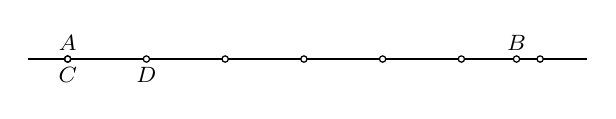
\begin{tikzpicture}
            % \clip (0,0) rectangle (14.000000,10.000000);
            {\footnotesize

            % Drawing line A B
            \draw [line width=0.016cm] (1.000000,1.500000) -- (1.460000,1.500000);%
            \draw [line width=0.016cm] (1.540000,1.500000) -- (2.460000,1.500000);%
            \draw [line width=0.016cm] (2.540000,1.500000) -- (3.460000,1.500000);%
            \draw [line width=0.016cm] (3.540000,1.500000) -- (4.460000,1.500000);%
            \draw [line width=0.016cm] (4.540000,1.500000) -- (5.460000,1.500000);%
            \draw [line width=0.016cm] (5.540000,1.500000) -- (6.460000,1.500000);%
            \draw [line width=0.016cm] (6.540000,1.500000) -- (7.160000,1.500000);%
            \draw [line width=0.016cm] (7.240000,1.500000) -- (7.460000,1.500000);%
            \draw [line width=0.016cm] (7.540000,1.500000) -- (8.100000,1.500000);%

            % Marking point A by circle
            \draw [line width=0.016cm] (1.500000,1.500000) circle (0.040000);%
            \draw (1.500000,1.500000) node [anchor=south] { $A$ };%

            % Marking point B by circle
            \draw [line width=0.016cm] (7.200000,1.500000) circle (0.040000);%
            \draw (7.200000,1.500000) node [anchor=south] { $B$ };%

            % Marking point C by circle
            \draw [line width=0.016cm] (1.500000,1.500000) circle (0.040000);%
            \draw (1.500000,1.500000) node [anchor=north] { $C$ };%

            % Marking point D by circle
            \draw [line width=0.016cm] (2.500000,1.500000) circle (0.040000);%
            \draw (2.500000,1.500000) node [anchor=north] { $D$ };%

            % Marking point E by circle
            \draw [line width=0.016cm] (3.500000,1.500000) circle (0.040000);%

            % Marking point F by circle
            \draw [line width=0.016cm] (4.500000,1.500000) circle (0.040000);%

            % Marking point G by circle
            \draw [line width=0.016cm] (5.500000,1.500000) circle (0.040000);%

            % Marking point H by circle
            \draw [line width=0.016cm] (6.500000,1.500000) circle (0.040000);%

            % Marking point I by circle
            \draw [line width=0.016cm] (7.500000,1.500000) circle (0.040000);%
            }
            \end{tikzpicture}
        \end{figure}
    \end{aksiom}

    % 
        Daljico $CD$, s katero smo izmerili daljico $AB$, imenujemo \textbf{enotska daljica}.
        Tako smo daljici $AB$ priredili natančno določeno število -- \textbf{dolžino} daljice $AB$ oziroma \textbf{razdaljo} točk $A$ in $B$.
        $$ |AB|=d(A,B)$$
    % 
    
        % Daljico $CD$ imenujemo \textbf{enotska daljica}.
        % Daljici $AB$ smo priredili natančno določeno število -- \textbf{dolžino} daljice $AB$ oziroma \textbf{razdaljo} točk $A$ in $B$.

        % $$ |AB|=d(A,B)$$
    





    \begin{aksiom}
        Če je $AB$ poljubna daljica, $A'$ pa točka na poljubnem poltraku, obstaja na tem poltraku natančno določena točka $B'$,
        da je daljica $A'B'$ skladna z daljico $AB$.

        $$A'B'\cong AB$$
    \end{aksiom}

    \begin{izrek}
        Skladni daljici imata enako dolžino.
        % $$|A'B'|=|AB|$$
    \end{izrek}

    ~ 

    \begin{aksiom}
        Naj daljici $AB$ in $BC$ ležita na isti premici in naj imata skupno le točko $B$.
        Daljici $A'B'$ in $B'C'$ naj ležita na tej ali neki drugi premici in naj imata skupno točko $B'$.
        Če velja $AB\cong A'B'$ in $BC\cong B'C'$, potem velja tudi $AC\cong A'C'$.
    \end{aksiom}

    \begin{izrek}
        Dolžina vsote daljic je enaka vsoti dolžin posameznih daljic.
    \end{izrek}




    \subsection*{Enote}


    
        Osnovna enota za merjenje dolžine je \textbf{meter}.

        Iz nje izpeljane enote pa so \textit{decimeter}, \textit{centimeter}, \textit{milimeter}, \textit{kilometer} itd.
        $$ 1~m=10~dm=100~cm=1000~mm$$  $$1~km=1000~m$$ 
    

    
        Enota za merjenje kotov je \textbf{kotna stopinja} -- velikost $\dfrac{1}{360}$ polnega kota.
        
        Izpeljani enoti sta \textit{(kotna) minuta} in \textit{(kotna) sekunda}.
        $$1^\circ=60'=3600''$$ 
    

    
        Velikost kota nič je $0^\circ$, pravega kota je $90^\circ$, iztegnjenega kota je $180^\circ$, polnega kota pa je $360^\circ$.
    

~


    \begin{definicija}
        Kota $\varphi$ in $\psi$, katerih vsota meri $180^\circ$, sta \textbf{suplementarna kota}.

        \begin{figure}[H]
            \centering
            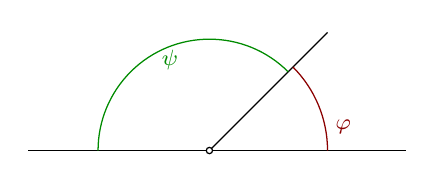
\begin{tikzpicture}
            % \clip (0,0) rectangle (14.000000,10.000000);
            {\footnotesize

            % Drawing line V P
            \draw [line width=0.016cm] (1.200000,1.500000) -- (3.460000,1.500000);%
            \draw [line width=0.016cm] (3.540000,1.500000) -- (6.000000,1.500000);%

            % Drawing line V Q
            % \draw [line width=0.016cm] (3.100000,1.100000) -- (3.471716,1.471716);%
            \draw [line width=0.016cm] (3.528284,1.528284) -- (5.000000,3.000000);%

            % Marking point V by circle
            \draw [line width=0.016cm] (3.500000,1.500000) circle (0.040000);%

            % Changing color 139 0 0
            \definecolor{r139g0b0}{rgb}{0.545098,0.000000,0.000000}%
            \color{r139g0b0}% 

            % Drawing arc V P 45.00
            \draw [line width=0.016cm] (5.000000,1.500000) arc (360:360:1.500000 and 1.500000) --(5.000000,1.500000) arc (0:45:1.500000 and 1.500000);%

            % Marking point \varphi
            \draw (5.200000,1.80000) node  { $\varphi$ };%

            % Changing color 0 139 0
            \definecolor{r0g139b0}{rgb}{0.000000,0.545098,0.000000}%
            \color{r0g139b0}% 

            % Drawing arc V Q 135.00
            \draw [line width=0.016cm] (4.500000,2.500000) arc (45:180:1.414214 and 1.414214);%

            % Marking point \psi
            \draw (3.000000,2.650000) node  { $\psi$ };%
            \color{black}
            }
            \end{tikzpicture}
        \end{figure}
    \end{definicija}

                
    \begin{definicija}
        Kota $\varphi$ in $\psi$, katerih vsota meri $90^\circ$, sta \textbf{komplementarna kota}.

        \begin{figure}[H]
            \centering
            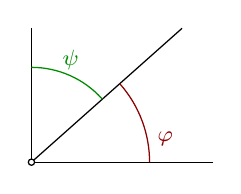
\begin{tikzpicture}
            % \clip (0,0) rectangle (14.000000,10.000000);
            {\footnotesize

            % Drawing line V P
            % \draw [line width=0.016cm] (2.800000,1.500000) -- (3.460000,1.500000);%
            \draw [line width=0.016cm] (3.540000,1.500000) -- (5.800000,1.500000);%

            % Drawing line V Q
            % \draw [line width=0.016cm] (3.050000,1.100000) -- (3.470104,1.473425);%
            \draw [line width=0.016cm] (3.529896,1.526575) -- (5.412500,3.200000);%

            % Drawing line V R
            % \draw [line width=0.016cm] (3.500000,1.100000) -- (3.500000,1.460000);%
            \draw [line width=0.016cm] (3.500000,1.540000) -- (3.500000,3.200000);%

            % Marking point V by circle
            \draw [line width=0.016cm] (3.500000,1.500000) circle (0.040000);%

            % Changing color 139 0 0
            \definecolor{r139g0b0}{rgb}{0.545098,0.000000,0.000000}%
            \color{r139g0b0}% 

            % Drawing arc V P 41.63
            \draw [line width=0.016cm] (5.000000,1.500000) arc (360:360:1.500000 and 1.500000) --(5.000000,1.500000) arc (0:41:1.500000 and 1.500000) -- (4.621114,2.496546);%

            % Marking point \varphi
            \draw (5.200000,1.800000) node  { $\varphi$ };%

            % Changing color 0 139 0
            \definecolor{r0g139b0}{rgb}{0.000000,0.545098,0.000000}%
            \color{r0g139b0}% 

            % Drawing arc V Q 48.37
            \draw [line width=0.016cm] (4.400000,2.300000) -- (4.394865,2.305740) arc (42:90:1.204159 and 1.204159);%

            % Marking point \psi
            \draw (4.000000,2.800000) node  { $\psi$ };%
            \color{black}
            }
            \end{tikzpicture}
        \end{figure}
    \end{definicija}

    
        Sokota sta vedno suplementarna kota.
    




    \subsection*{Skladnost trikotnikov}


    \begin{definicija}
        Dva trikotnika sta \textbf{skladna}, če imata paroma skladne vse stranice in tem stranicam nasprotne kote.
    \end{definicija}

    \begin{aksiom}
        Dva trikotnika sta skladna, če se ujemata v dveh stranicah in v vmesnem kotu.
    \end{aksiom}

    \begin{izrek}
        Trikotnika $\triangle ABC$ in $\triangle A'B'C'$ sta skladna, če se ujemata:
        \begin{enumerate}
            \item v vseh treh stranicah;
            \item v eni stranici in obeh priležnih kotih;
            \item v dveh stranicah in kotu, ki leži nasproti daljši od obeh stranic.
        \end{enumerate}
    \end{izrek}




%%%% naloge


~\\~~\\~\\


    \begin{naloga}
        Izračunajte dolžino daljice, če ena polovica meri $2x-7$ enot, druga polovica pa $x+8$ enot.
    \end{naloga}

    \begin{naloga}
        Izračunaj dolžino $x$ daljice $AB$, če je točka $S$ njeno razpolovišče, točka $R$ pa razpolovišče daljice $SB$ in je $\lvert SR \rvert = \dfrac{x}{3}-1$.
    \end{naloga}

    \begin{naloga}
        Izračunajte velikosti kotov $\angle AVM$ in $\angle FVE$, če poltrak $VM$ obakrat razpolavlja kot.

        \begin{figure}[H]
            \centering
            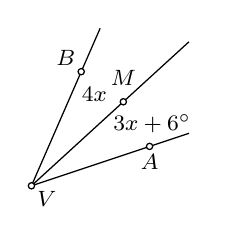
\begin{tikzpicture}
                % \clip (0,0) rectangle (14.000000,10.000000);
                {\footnotesize

                % Marking point V by circle
                \draw [line width=0.016cm] (1.500000,1.500000) circle (0.040000);%
                \draw (1.470000,1.530000) node [anchor=north west] { $V$ };%

                % Marking point A by circle
                \draw [line width=0.016cm] (3.000000,2.000000) circle (0.040000);%
                \draw (3.000000,2.000000) node [anchor=north] { $A$ };%

                % Drawing line V A
                % \draw [line width=0.016cm] (1.200000,1.400000) -- (1.462053,1.487351);%
                \draw [line width=0.016cm] (1.537947,1.512649) -- (2.962053,1.987351);%
                \draw [line width=0.016cm] (3.037947,2.012649) -- (3.500000,2.166667);%

                % Marking point M by circle
                \draw [line width=0.016cm] (2.666950,2.566878) circle (0.040000);%
                \draw (2.666950,2.666878) node [anchor=south] { $M$ };%

                % Marking point B by circle
                \draw [line width=0.016cm] (2.132124,2.949283) circle (0.040000);%
                \draw (2.162124,2.919283) node [anchor=south east] { $B$ };%

                % Drawing line V B
                % \draw [line width=0.016cm] (1.369151,1.200000) -- (1.484008,1.463336);%
                \draw [line width=0.016cm] (1.515992,1.536664) -- (2.116132,2.912618);%
                \draw [line width=0.016cm] (2.148115,2.985947) -- (2.372326,3.500000);%

                % Drawing line V M
                % \draw [line width=0.016cm] (1.200000,1.225727) -- (1.470478,1.473010);%
                \draw [line width=0.016cm] (1.529522,1.526990) -- (2.637428,2.539888);%
                \draw [line width=0.016cm] (2.696472,2.593868) -- (3.500000,3.328489);%

                % Marking point {3x+6^\circ}
                \draw (3.033475,2.283439) node  { ${3x+6^\circ}$ };%

                % Marking point {4x}
                \draw (2.299537,2.658080) node  { ${4x}$ };%
                }
            \end{tikzpicture} ~
            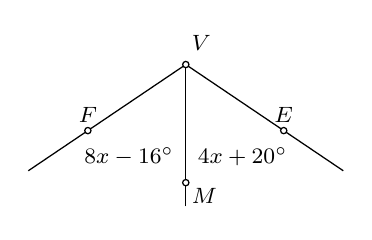
\begin{tikzpicture}
                % \clip (0,0) rectangle (14.000000,10.000000);
                {\footnotesize

                % Marking point V by circle
                \draw [line width=0.016cm] (4.000000,4.000000) circle (0.040000);%
                \draw (3.970000,4.070000) node [anchor=south west] { $V$ };%

                % Marking point M by circle
                \draw [line width=0.016cm] (4.000000,2.500000) circle (0.040000);%
                \draw (3.970000,2.530000) node [anchor=north west] { $M$ };%

                % Drawing line V M
                \draw [line width=0.016cm] (4.000000,2.200000) -- (4.000000,2.460000);%
                \draw [line width=0.016cm] (4.000000,2.540000) -- (4.000000,3.960000);%
                % \draw [line width=0.016cm] (4.000000,4.040000) -- (4.000000,4.200000);%

                % Marking point F by circle
                \draw [line width=0.016cm] (2.756444,3.161211) circle (0.040000);%
                \draw (2.756444,3.161211) node [anchor=south] { $F$ };%

                % Marking point E by circle
                \draw [line width=0.016cm] (5.243556,3.161211) circle (0.040000);%
                \draw (5.243556,3.161211) node [anchor=south] { $E$ };%

                % Drawing line V E
                % \draw [line width=0.016cm] (3.703488,4.200000) -- (3.966838,4.022368);%
                \draw [line width=0.016cm] (4.033162,3.977632) -- (5.210395,3.183578);%
                \draw [line width=0.016cm] (5.276718,3.138843) -- (6.000000,2.650983);%

                % Drawing line V F
                % \draw [line width=0.016cm] (4.296512,4.200000) -- (4.033162,4.022368);%
                \draw [line width=0.016cm] (3.966838,3.977632) -- (2.789605,3.183578);%
                \draw [line width=0.016cm] (2.723282,3.138843) -- (2.000000,2.650983);%

                % Marking point {8x-16^\circ}
                \draw (3.278222,2.830605) node  { ${8x-16^\circ}$ };%

                % Marking point {4x+20^\circ}
                \draw (4.721778,2.830605) node  { ${4x+20^\circ}$ };%
                }
            \end{tikzpicture}


        \end{figure}
    \end{naloga}


    \begin{multicols}{2}
    \begin{naloga}
        Izračunajte velikosti kotov $\alpha$ in $\beta$, če je $\alpha=\beta$.
        Podatke razberite s skice.

        \begin{figure}[H]
            \centering
            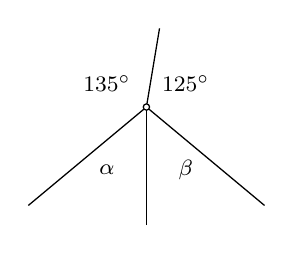
\begin{tikzpicture}
                % \clip (0,0) rectangle (14.000000,10.000000);
                {\footnotesize

                % Marking point A by circle
                \draw [line width=0.016cm] (3.000000,3.000000) circle (0.040000);%

                % Drawing segment A B
                \draw [line width=0.016cm] (3.000000,1.500000) -- (3.000000,2.960000);%

                % Drawing segment A C
                \draw [line width=0.016cm] (3.030729,2.974393) -- (4.500000,1.750000);%

                % Drawing segment A D
                \draw [line width=0.016cm] (2.969271,2.974393) -- (1.500000,1.750000);%

                % Drawing segment A E
                \draw [line width=0.016cm] (3.006576,3.039456) -- (3.166667,4.000000);%

                % Marking point \beta
                \draw (3.500000,2.200000) node  { $\beta$ };%

                % Marking point \alpha
                \draw (2.500000,2.200000) node  { $\alpha$ };%

                % Marking point {125^\circ}
                \draw (3.500000,3.300000) node  { ${125^\circ}$ };%

                % Marking point {135^\circ}
                \draw (2.500000,3.300000) node  { ${135^\circ}$ };%
                }
            \end{tikzpicture}

        \end{figure}
    \end{naloga}




    \begin{naloga}
        Iz podatkov na skici izračunajte neznano velikost kota $x$.

        \begin{figure}[H]
            \centering
            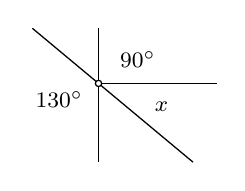
\begin{tikzpicture}
                % \clip (0,0) rectangle (14.000000,10.000000);
                {\footnotesize

                % Marking point A by circle
                \draw [line width=0.016cm] (3.000000,3.000000) circle (0.040000);%

                % Drawing line A B
                \draw [line width=0.016cm] (3.000000,2.000000) -- (3.000000,2.960000);%
                \draw [line width=0.016cm] (3.000000,3.040000) -- (3.000000,3.700000);%

                % Drawing line A C
                \draw [line width=0.016cm] (4.200000,2.000000) -- (3.030729,2.974393);%
                \draw [line width=0.016cm] (2.969271,3.025607) -- (2.160000,3.700000);%

                % Drawing segment A E
                \draw [line width=0.016cm] (3.040000,3.000000) -- (4.500000,3.000000);%

                % Marking point x
                \draw (3.800000,2.700000) node  { $x$ };%

                % Marking point {90^\circ}
                \draw (3.500000,3.300000) node  { ${90^\circ}$ };%

                % Marking point {130^\circ}
                \draw (2.500000,2.800000) node  { ${130^\circ}$ };%
                }
            \end{tikzpicture}

        \end{figure}
    \end{naloga}

\end{multicols}





    \begin{multicols}{2}
        
    \begin{naloga}
        Izračunajte velikost kota $\angle PVQ$, če je $\angle PVR=94^\circ$.

        \begin{figure}[H]
            \centering
            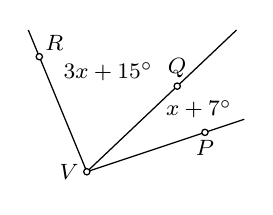
\begin{tikzpicture}
                % \clip (0,0) rectangle (14.000000,10.000000);
                {\footnotesize

                % Marking point V by circle
                \draw [line width=0.016cm] (3.500000,1.500000) circle (0.040000);%
                \draw (3.500000,1.500000) node [anchor=east] { $V$ };%

                % Marking point P by circle
                \draw [line width=0.016cm] (5.000000,2.000000) circle (0.040000);%
                \draw (5.000000,2.000000) node [anchor=north] { $P$ };%

                % Drawing line V P
                % \draw [line width=0.016cm] (2.600000,1.200000) -- (3.462053,1.487351);%
                \draw [line width=0.016cm] (3.537947,1.512649) -- (4.962053,1.987351);%
                \draw [line width=0.016cm] (5.037947,2.012649) -- (5.500000,2.166667);%

                % Marking point Q by circle
                \draw [line width=0.016cm] (4.648153,2.587081) circle (0.040000);%
                \draw (4.648153,2.587081) node [anchor=south] { $Q$ };%

                % Marking point R by circle
                \draw [line width=0.016cm] (2.896583,2.961468) circle (0.040000);%
                \draw (2.866583,2.931468) node [anchor=south west] { $R$ };%

                % Drawing line V R
                % \draw [line width=0.016cm] (3.623865,1.200000) -- (3.515265,1.463027);%
                \draw [line width=0.016cm] (3.484735,1.536973) -- (2.911849,2.924495);%
                \draw [line width=0.016cm] (2.881318,2.998440) -- (2.756809,3.300000);%

                % Drawing line V Q
                % \draw [line width=0.016cm] (3.183146,1.200000) -- (3.470954,1.472499);%
                \draw [line width=0.016cm] (3.529046,1.527501) -- (4.619106,2.559580);%
                \draw [line width=0.016cm] (4.677199,2.614582) -- (5.401122,3.300000);%

                % Marking point {x+7^\circ}
                \draw (4.924076,2.293541) node  { ${x+7^\circ}$ };%

                % Marking point {3x+15^\circ}
                \draw (3.772368,2.774275) node  { ${3x+15^\circ}$ };%
                }
            \end{tikzpicture}

        \end{figure}
    \end{naloga}


    \begin{naloga}
        Izračunajte velikost kota $\angle SVR$, če je $\angle QVS=50^\circ$.

        \begin{figure}[H]
            \centering
            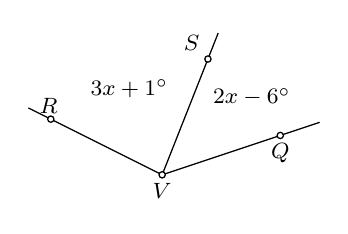
\begin{tikzpicture}
                % \clip (0,0) rectangle (14.000000,10.000000);
                {\footnotesize

                % Marking point V by circle
                \draw [line width=0.016cm] (3.500000,1.500000) circle (0.040000);%
                \draw (3.500000,1.500000) node [anchor=north] { $V$ };%

                % Marking point P by circle
                \draw [line width=0.016cm] (5.000000,2.000000) circle (0.040000);%
                \draw (5.000000,2.000000) node [anchor=north] { $Q$ };%

                % Drawing line V P
                % \draw [line width=0.016cm] (2.600000,1.200000) -- (3.462053,1.487351);%
                \draw [line width=0.016cm] (3.537947,1.512649) -- (4.962053,1.987351);%
                \draw [line width=0.016cm] (5.037947,2.012649) -- (5.500000,2.166667);%

                % Marking point S by circle
                \draw [line width=0.016cm] (4.081159,2.970460) circle (0.040000);%
                \draw (4.081159,2.970460) node [anchor=south east] { $S$ };%

                % Marking point R by circle
                \draw [line width=0.016cm] (2.085787,2.207107) circle (0.040000);%
                \draw (2.055787,2.177107) node [anchor=south] { $R$ };%

                % Drawing line V R
                % \draw [line width=0.016cm] (4.100000,1.200000) -- (3.535777,1.482111);%
                \draw [line width=0.016cm] (3.464223,1.517889) -- (2.121564,2.189218);%
                \draw [line width=0.016cm] (2.050009,2.224995) -- (1.800000,2.350000);%

                % Drawing line V S
                % \draw [line width=0.016cm] (3.381433,1.200000) -- (3.485298,1.462800);%
                \draw [line width=0.016cm] (3.514702,1.537200) -- (4.066457,2.933260);%
                \draw [line width=0.016cm] (4.095862,3.007660) -- (4.211401,3.300000);%

                % Marking point {2x-6^\circ}
                \draw (4.640580,2.485230) node  { ${2x-6^\circ}$ };%

                % Marking point {3x+1^\circ}
                \draw (3.083473,2.588784) node  { ${3x+1^\circ}$ };%
                }
            \end{tikzpicture}

        \end{figure}
    \end{naloga}


    \end{multicols}

        


    \begin{naloga}
        Kot $\varphi=76^\circ 36'53''$ zapišite v stopinjah na štiri mesta natančno, 
        kot $\psi=34.78^\circ$ pa zapišite v stopinjah, minutah in sekundah.
    \end{naloga}

    \begin{naloga}
        Kotu $\varphi=37^\circ 16'43''$ izračunajte suplementarni in komplementarni kot.
    \end{naloga}

    \begin{naloga}
        Razika dveh komplementarnih kotov je $37^\circ 16'$. Izračunajte velikosti kotov.
    \end{naloga}

    \begin{naloga}
        Izračunajte velikost kota $\varphi$, ki je petkratnik svojega komplementarnega kota.
    \end{naloga}





    \begin{naloga}
        Za vsako od spodnjih izjav ugotovite, ali je pravilna ali nepravilna.
        \begin{itemize}
            \item Sokota sta suplementarna.
            % \item Kota z vzporednimi kraki sta skladna.
            \item Kot z velikostjo $45^\circ$ je komplementaren samemu sebi.
            \item Dve premici, ki se sekata, lahko določata kota z velikostjo $43^\circ$ in $137^\circ$.
            \item Vsota velikosti dveh komplementarnih kotov je pravi kot.
            \item Suplementarna kota sta  vedno tudi sokota.
        \end{itemize}
    \end{naloga}

    \begin{naloga}
        Poltrak $VD$ razpolavlja $\angle CVE$, $\angle BVC$ je pravi kot.
        Določite velikosti kotov $\angle AVD$ in $\angle BVE$.

        \begin{figure}[H]
            \centering
            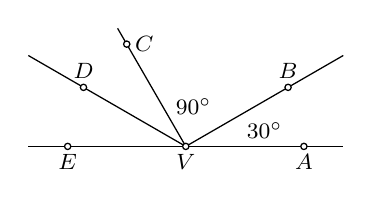
\begin{tikzpicture}
                % \clip (0,0) rectangle (14.000000,10.000000);
                {\footnotesize

                % Marking point V by circle
                \draw [line width=0.016cm] (4.000000,1.500000) circle (0.040000);%
                \draw (4.000000,1.500000) node [anchor=north] { $V$ };%

                % Marking point A by circle
                \draw [line width=0.016cm] (5.500000,1.500000) circle (0.040000);%
                \draw (5.500000,1.500000) node [anchor=north] { $A$ };%

                % Marking point E by circle
                \draw [line width=0.016cm] (2.500000,1.500000) circle (0.040000);%
                \draw (2.500000,1.500000) node [anchor=north] { $E$ };%

                % Drawing line A E
                \draw [line width=0.016cm] (2.000000,1.500000) -- (2.460000,1.500000);%
                \draw [line width=0.016cm] (2.540000,1.500000) -- (3.960000,1.500000);%
                \draw [line width=0.016cm] (4.040000,1.500000) -- (5.460000,1.500000);%
                \draw [line width=0.016cm] (5.540000,1.500000) -- (6.000000,1.500000);%

                % Marking point B by circle
                \draw [line width=0.016cm] (5.299038,2.250000) circle (0.040000);%
                \draw (5.299038,2.250000) node [anchor=south] { $B$ };%

                % Marking point C by circle
                \draw [line width=0.016cm] (3.250000,2.799038) circle (0.040000);%
                \draw (3.250000,2.799038) node [anchor=west] { $C$ };%

                % Marking point D by circle
                \draw [line width=0.016cm] (2.700962,2.250000) circle (0.040000);%
                \draw (2.700962,2.250000) node [anchor=south] { $D$ };%

                % Drawing line V D
                % \draw [line width=0.016cm] (4.519615,1.200000) -- (4.034641,1.480000);%
                \draw [line width=0.016cm] (3.965359,1.520000) -- (2.735603,2.230000);%
                \draw [line width=0.016cm] (2.666321,2.270000) -- (2.000000,2.654701);%

                % Drawing line V C
                % \draw [line width=0.016cm] (4.173205,1.200000) -- (4.020000,1.465359);%
                \draw [line width=0.016cm] (3.980000,1.534641) -- (3.270000,2.764397);%
                \draw [line width=0.016cm] (3.230000,2.833679) -- (3.133975,3.000000);%

                % Drawing line V B
                % \draw [line width=0.016cm] (3.480385,1.200000) -- (3.965359,1.480000);%
                \draw [line width=0.016cm] (4.034641,1.520000) -- (5.264397,2.230000);%
                \draw [line width=0.016cm] (5.333679,2.270000) -- (6.000000,2.654700);%

                % Marking point {30^\circ}
                \draw (5.000000,1.500000) node [anchor=south] { ${30^\circ}$ };%

                % Marking point {90^\circ}
                \draw (4.100000,1.800000) node [anchor=south] { ${90^\circ}$ };%
                }
            \end{tikzpicture}

        \end{figure}
    \end{naloga}






\newpage
%%%%%%%%%%%%%%%%%%%%%%%%%%%%%%%%%%%%%%%


\section{Vzporednost in pravokotnost}

    \subsection*{Vzporednost}
            
            \begin{aksiom}[Aksiom o vzporednici]
                Skozi izbrano točko, ki ne leži na premici, lahko tej premici načrtamo natanko eno vzporednico.

                \begin{figure}[H]
                    \centering
                    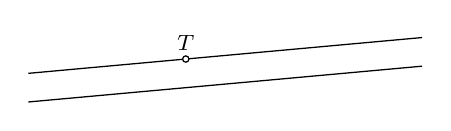
\begin{tikzpicture}
                    % \clip (0,0) rectangle (14.000000,10.000000);
                    {\footnotesize

                    % Drawing line p
                    \draw [line width=0.016cm] (1.000000,1.454545) -- (6.000000,1.909091);%

                    % Drawing line q
                    \draw [line width=0.016cm] (1.000000,1.818182) -- (2.960164,1.996379);%
                    \draw [line width=0.016cm] (3.039836,2.003621) -- (6.000000,2.272727);%

                    % Marking point T by circle
                    \draw [line width=0.016cm] (3.000000,2.000000) circle (0.040000);%
                    \draw (3.000000,2.000000) node [anchor=south] { $T$ };%
                    }
                    \end{tikzpicture}

                \end{figure}

            \end{aksiom}

            
                \textbf{Vzporednost} je v množici premic na ravnini \textit{ekvivalenčna relacija}, saj je:
                \begin{itemize}
                    \item \textit{refleksivna}: $p\parallel p$ -- vsaka premica je vzporedna sama sebi;
                    \item \textit{simetrična}: $p\parallel q \Rightarrow q\parallel p$ -- če je premica $p$ vzporedna premici $q$, je tudi premica $q$ vzporedna premici $p$;
                    \item \textit{tranzitivna}: $p\parallel q \land q \parallel r \rightarrow p \parallel r$ -- če je premica $p$ vzporedna premici $q$, premica $q$ pa vzporedna premici $r$, 
                        je tudi premica $p$ vzporedna premici $r$.
                \end{itemize}

                ~
        
            
                Če vzporednici sekamo s premico, dobimo dve presečišči, ob njiju pa pare \textbf{kotov z vzporednimi kraki}:
                

                \begin{itemize}
                    \item pari kotov $(\alpha, \gamma)$, $(\beta, \delta)$, $(\alpha', \gamma')$, $(\beta', \delta')$ imajo oba kraka vzporedna v isto smer;
                    \item pari kotov z istim vrhom $(\alpha, \beta)$; $(\gamma, \delta)$, $(\alpha', \beta')$; $(\gamma', \delta')$ imajo oba kraka vzporedna v nasprotno smer -- \textbf{sovršni koti};
                    \item pari kotov $(\alpha, \alpha')$, $(\beta, \beta')$, $(\gamma,\gamma')$, $(\delta,\delta')$ imajo en krak vzporeden v isto smer, drugi krak pa vzporeden v nasprotno smer.
                \end{itemize}

                \begin{figure}[H]
                    \centering
                    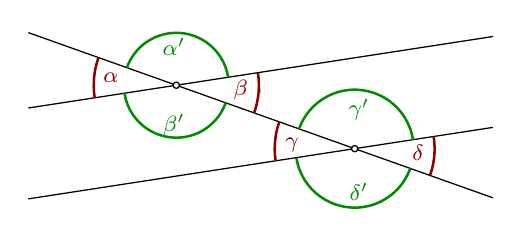
\begin{tikzpicture}
                    % \clip (0,0) rectangle (14.000000,10.000000);
                    {\footnotesize

                    % Drawing line p
                    \draw [line width=0.016cm] (1.300000,1.315385) -- (5.405096,1.946938);%
                    \draw [line width=0.016cm] (5.484166,1.959102) -- (7.200000,2.223077);%

                    % Drawing line q
                    \draw [line width=0.016cm] (1.300000,2.469231) -- (3.139995,2.752307);%
                    \draw [line width=0.016cm] (3.219065,2.764472) -- (7.200000,3.376923);%

                    % Drawing line r
                    \draw [line width=0.016cm] (1.300000,3.426667) -- (3.141842,2.771790);%
                    \draw [line width=0.016cm] (3.217219,2.744989) -- (5.406942,1.966421);%
                    \draw [line width=0.016cm] (5.482319,1.939620) -- (7.200000,1.328889);%

                    % Marking point U by circle
                    \draw [line width=0.016cm] (5.444631,1.953020) circle (0.040000);%

                    % Marking point V by circle
                    \draw [line width=0.016cm] (3.179530,2.758389) circle (0.040000);%

                    % Changing color 139 0 0
                    \definecolor{r139g0b0}{rgb}{0.545098,0.000000,0.000000}%
                    \color{r139g0b0}% 

                    % Drawing arc V L 28.32
                    \draw [line width=0.032cm] (2.191446,3.109708) -- (2.187982,3.099807) arc (161:188:1.048682 and 1.048682) -- (2.143042,2.598930);%

                    % Drawing arc V M 28.32
                    \draw [line width=0.032cm] (4.167614,2.407070) -- (4.171079,2.416971) arc (341:360:1.048682 and 1.048682) --(4.228212,2.758389) arc (0:8:1.048682 and 1.048682) -- (4.216018,2.917849);%

                    % Drawing arc U N 28.32
                    \draw [line width=0.032cm] (4.487996,2.293157) -- (4.484642,2.283571) arc (161:188:1.015305 and 1.015305) -- (4.441133,1.798636);%

                    % Drawing arc U O 28.32
                    \draw [line width=0.032cm] (6.401266,1.612883) -- (6.404620,1.622469) arc (341:360:1.015305 and 1.015305) --(6.459935,1.953020) arc (0:8:1.015305 and 1.015305) -- (6.448129,2.107404);%

                    % Marking point \alpha
                    \draw (2.350000,2.850000) node  { $\alpha$ };%

                    % Marking point \beta
                    \draw (4.000000,2.700000) node  { $\beta$ };%

                    % Marking point \gamma
                    \draw (4.650000,2.000000) node  { $\gamma$ };%

                    % Marking point \delta
                    \draw (6.250000,1.900000) node  { $\delta$ };%

                    % Changing color 0 139 0
                    \definecolor{r0g139b0}{rgb}{0.000000,0.545098,0.000000}%
                    \color{r0g139b0}% 

                    % Drawing arc V J 151.68
                    \draw [line width=0.032cm] (3.837639,2.859637) -- (3.837184,2.862551) arc (9:160:0.665852 and 0.665852) -- (2.552155,2.981456);%

                    % Drawing arc V K 151.68
                    \draw [line width=0.032cm] (2.521421,2.657142) -- (2.521876,2.654227) arc (189:340:0.665852 and 0.665852) -- (3.806905,2.535322);%

                    % Drawing arc U P 151.68
                    \draw [line width=0.032cm] (6.184950,2.066915) -- (6.184438,2.070194) arc (9:160:0.749029 and 0.749029) -- (4.738885,2.203952);%

                    % Drawing arc U R 151.68
                    \draw [line width=0.032cm] (4.704312,1.839125) -- (4.704824,1.835846) arc (189:340:0.749029 and 0.749029) -- (6.150377,1.702088);%

                    % Marking point \alpha'
                    \draw (3.150000,3.250000) node  { $\alpha'$ };%

                    % Marking point \beta'
                    \draw (3.150000,2.250000) node  { $\beta'$ };%

                    % Marking point \gamma'
                    \draw (5.500000,2.450000) node  { $\gamma'$ };%

                    % Marking point \delta'
                    \draw (5.500000,1.400000) node  { $\delta'$ };%
                    \color{black}
                    }
                    \end{tikzpicture}
                    
                \end{figure}



        
            \begin{izrek}
                Para konveksnih kotov z vzporednimi kraki sta bodisi skladna bodisi suplementarna.

                \begin{figure}[H]
                    \centering
                    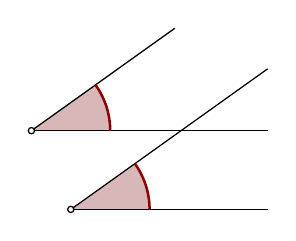
\begin{tikzpicture}
                    % \clip (0,0) rectangle (14.000000,10.000000);
                    {\footnotesize

                    % Changing color 215 183 183
                    \definecolor{r215g183b183}{rgb}{0.843137,0.717647,0.717647}%
                    \color{r215g183b183}% 

                    % Filling circle arc V D 35.54
                    \fill (1.500000,2.500000) -- (2.500000,2.500000) arc (0:35:1.000000 and 1.000000) -- (2.313733,3.081238) -- cycle;%

                    % Filling circle arc U E 35.54
                    \fill (2.000000,1.500000) -- (3.000000,1.500000) arc (0:35:1.000000 and 1.000000) -- (2.813733,2.081238) -- cycle;%

                    % Changing color 0 0 0
                    \definecolor{r0g0b0}{rgb}{0.000000,0.000000,0.000000}%
                    \color{r0g0b0}% 

                    % Marking point V by circle
                    \draw [line width=0.016cm] (1.500000,2.500000) circle (0.040000);%

                    % Drawing line V A
                    % \draw [line width=0.016cm] (1.000000,2.500000) -- (1.460000,2.500000);%
                    \draw [line width=0.016cm] (1.540000,2.500000) -- (4.500000,2.500000);%

                    % Drawing line V B
                    \draw [line width=0.016cm] (3.320000,3.800000) -- (1.532549,2.523250);%
                    % \draw [line width=0.016cm] (1.467451,2.476750) -- (1.000000,2.142857);%

                    % Marking point U by circle
                    \draw [line width=0.016cm] (2.000000,1.500000) circle (0.040000);%

                    % Drawing line r
                    % \draw [line width=0.016cm] (1.300000,1.000000) -- (1.967451,1.476750);%
                    \draw [line width=0.016cm] (2.032549,1.523250) -- (4.500000,3.285714);%

                    % Drawing line s
                    % \draw [line width=0.016cm] (1.000000,1.500000) -- (1.960000,1.500000);%
                    \draw [line width=0.016cm] (2.040000,1.500000) -- (4.500000,1.500000);%

                    % Changing color 139 0 0
                    \definecolor{r139g0b0}{rgb}{0.545098,0.000000,0.000000}%
                    \color{r139g0b0}% 

                    % Drawing arc V D 35.54
                    \draw [line width=0.032cm] (2.500000,2.500000) arc (360:360:1.000000 and 1.000000) --(2.500000,2.500000) arc (0:35:1.000000 and 1.000000) -- (2.313733,3.081238);%

                    % Drawing arc U E 35.54
                    \draw [line width=0.032cm] (3.000000,1.500000) arc (360:360:1.000000 and 1.000000) --(3.000000,1.500000) arc (0:35:1.000000 and 1.000000) -- (2.813733,2.081238);%
                    \color{black}
                    }
                    \end{tikzpicture} ~~~~
                    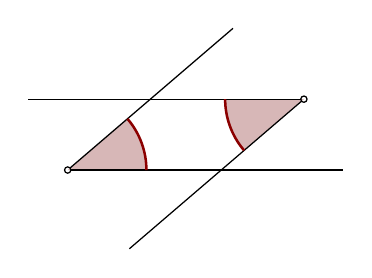
\begin{tikzpicture}
                    % \clip (0,0) rectangle (14.000000,10.000000);
                    {\footnotesize

                    % Changing color 215 183 183
                    \definecolor{r215g183b183}{rgb}{0.843137,0.717647,0.717647}%
                    \color{r215g183b183}% 

                    % Filling circle arc V D 40.60
                    \fill (1.500000,2.000000) -- (2.500000,2.000000) arc (0:40:1.000000 and 1.000000) -- (2.259257,2.650791) -- cycle;%

                    % Filling circle arc U E 40.60
                    \fill (4.500000,2.900000) -- (3.500000,2.900000) arc (180:220:1.000000 and 1.000000) -- (3.740743,2.249209) -- cycle;%

                    % Changing color 0 0 0
                    \definecolor{r0g0b0}{rgb}{0.000000,0.000000,0.000000}%
                    \color{r0g0b0}% 

                    % Marking point V by circle
                    \draw [line width=0.016cm] (1.500000,2.000000) circle (0.040000);%

                    % Drawing line V A
                    % \draw [line width=0.016cm] (1.000000,2.000000) -- (1.460000,2.000000);%
                    \draw [line width=0.016cm] (1.540000,2.000000) -- (5.000000,2.000000);%

                    % Drawing line V B
                    \draw [line width=0.016cm] (3.600000,3.800000) -- (1.530370,2.026032);%
                    % \draw [line width=0.016cm] (1.469630,1.973968) -- (1.000000,1.571429);%

                    % Marking point U by circle
                    \draw [line width=0.016cm] (4.500000,2.900000) circle (0.040000);%

                    % Drawing line r
                    \draw [line width=0.016cm] (2.283333,1.000000) -- (4.469630,2.873968);%
                    % \draw [line width=0.016cm] (4.530370,2.926032) -- (5.000000,3.328571);%

                    % Drawing line s
                    \draw [line width=0.016cm] (1.000000,2.900000) -- (4.460000,2.900000);%
                    % \draw [line width=0.016cm] (4.540000,2.900000) -- (5.000000,2.900000);%

                    % Changing color 139 0 0
                    \definecolor{r139g0b0}{rgb}{0.545098,0.000000,0.000000}%
                    \color{r139g0b0}% 

                    % Drawing arc V D 40.60
                    \draw [line width=0.032cm] (2.500000,2.000000) arc (360:360:1.000000 and 1.000000) --(2.500000,2.000000) arc (0:40:1.000000 and 1.000000) -- (2.259257,2.650791);%

                    % Drawing arc U E 40.60
                    \draw [line width=0.032cm] (3.500000,2.900000) arc (180:220:1.000000 and 1.000000) -- (3.740743,2.249209);%
                    \color{black}
                    }
                    \end{tikzpicture} ~~~~
                    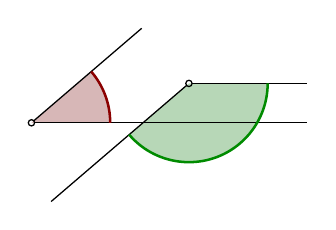
\begin{tikzpicture}
                    % \clip (0,0) rectangle (14.000000,10.000000);
                    {\footnotesize

                    % Changing color 215 183 183
                    \definecolor{r215g183b183}{rgb}{0.843137,0.717647,0.717647}%
                    \color{r215g183b183}% 

                    % Filling circle arc V D 40.60
                    \fill (1.500000,2.000000) -- (2.500000,2.000000) arc (0:40:1.000000 and 1.000000) -- (2.259257,2.650791) -- cycle;%

                    % Changing color 183 215 183
                    \definecolor{r183g215b183}{rgb}{0.717647,0.843137,0.717647}%
                    \color{r183g215b183}% 

                    % Filling circle arc U G 139.40
                    \fill (3.500000,2.500000) -- (2.740743,1.849209) -- (2.745290,1.843941) arc (221:360:1.000000 and 1.000000) --(4.500000,2.500000) arc (0:0:1.000000 and 1.000000) -- cycle;%

                    % Changing color 0 0 0
                    \definecolor{r0g0b0}{rgb}{0.000000,0.000000,0.000000}%
                    \color{r0g0b0}% 

                    % Marking point V by circle
                    \draw [line width=0.016cm] (1.500000,2.000000) circle (0.040000);%

                    % Drawing line V A
                    % \draw [line width=0.016cm] (1.000000,2.000000) -- (1.460000,2.000000);%
                    \draw [line width=0.016cm] (1.540000,2.000000) -- (5.000000,2.000000);%

                    % Drawing line V B
                    \draw [line width=0.016cm] (2.900000,3.200000) -- (1.530370,2.026032);%
                    % \draw [line width=0.016cm] (1.469630,1.973968) -- (1.000000,1.571429);%

                    % Marking point U by circle
                    \draw [line width=0.016cm] (3.500000,2.500000) circle (0.040000);%

                    % Drawing line r
                    \draw [line width=0.016cm] (1.750000,1.000000) -- (3.469630,2.473968);%
                    % \draw [line width=0.016cm] (3.530370,2.526032) -- (4.316667,3.200000);%

                    % Drawing line s
                    % \draw [line width=0.016cm] (1.000000,2.500000) -- (3.460000,2.500000);%
                    \draw [line width=0.016cm] (3.540000,2.500000) -- (5.000000,2.500000);%

                    % Changing color 139 0 0
                    \definecolor{r139g0b0}{rgb}{0.545098,0.000000,0.000000}%
                    \color{r139g0b0}% 

                    % Drawing arc V D 40.60
                    \draw [line width=0.032cm] (2.500000,2.000000) arc (360:360:1.000000 and 1.000000) --(2.500000,2.000000) arc (0:40:1.000000 and 1.000000) -- (2.259257,2.650791);%

                    % Changing color 0 139 0
                    \definecolor{r0g139b0}{rgb}{0.000000,0.545098,0.000000}%
                    \color{r0g139b0}% 

                    % Drawing arc U G 139.40
                    \draw [line width=0.032cm] (2.740743,1.849209) -- (2.745290,1.843941) arc (221:360:1.000000 and 1.000000);%
                    \color{black}
                    }
                    \end{tikzpicture}

                \end{figure}
            \end{izrek}

            
                Sovršna kota sta skladna -- imata isti sokot.

                \begin{figure}[H]
                    \centering
                    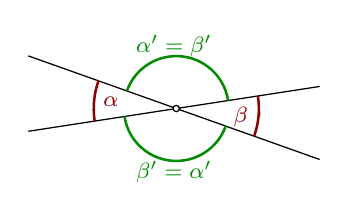
\begin{tikzpicture}
                    % \clip (0,0) rectangle (14.000000,10.000000);
                    {\footnotesize

                    % Drawing line p

                    % Drawing line q
                    \draw [line width=0.016cm] (1.300000,2.469231) -- (3.139995,2.752307);%
                    \draw [line width=0.016cm] (3.219065,2.764472) -- (5.000000,3.038462);%

                    % Drawing line r
                    \draw [line width=0.016cm] (1.300000,3.426667) -- (3.141842,2.771790);%
                    \draw [line width=0.016cm] (3.217219,2.744989) -- (5.000000,2.111111);%

                    % Marking point U by circle

                    % Marking point V by circle
                    \draw [line width=0.016cm] (3.179530,2.758389) circle (0.040000);%

                    % Changing color 139 0 0
                    \definecolor{r139g0b0}{rgb}{0.545098,0.000000,0.000000}%
                    \color{r139g0b0}% 

                    % Drawing arc V L 28.32
                    \draw [line width=0.032cm] (2.191446,3.109708) -- (2.187982,3.099807) arc (161:188:1.048682 and 1.048682) -- (2.143042,2.598930);%

                    % Drawing arc V M 28.32
                    \draw [line width=0.032cm] (4.167614,2.407070) -- (4.171079,2.416971) arc (341:360:1.048682 and 1.048682) --(4.228212,2.758389) arc (0:8:1.048682 and 1.048682) -- (4.216018,2.917849);%

                    % Marking point \alpha
                    \draw (2.350000,2.850000) node  { $\alpha$ };%

                    % Marking point \beta
                    \draw (4.000000,2.650000) node  { $\beta$ };%

                    % Changing color 0 139 0
                    \definecolor{r0g139b0}{rgb}{0.000000,0.545098,0.000000}%
                    \color{r0g139b0}% 

                    % Drawing arc V J 151.68
                    \draw [line width=0.032cm] (3.837639,2.859637) -- (3.837184,2.862551) arc (9:160:0.665852 and 0.665852) -- (2.552155,2.981456);%

                    % Drawing arc V K 151.68
                    \draw [line width=0.032cm] (2.521421,2.657142) -- (2.521876,2.654227) arc (189:340:0.665852 and 0.665852) -- (3.806905,2.535322);%

                    % Marking point \alpha'
                    \draw (3.150000,3.55000) node  { $\alpha'=\beta'$ };%

                    % Marking point \beta'
                    \draw (3.150000,1.95000) node  { $\beta'=\alpha'$ };%
                    \color{black}
                    }
                    \end{tikzpicture}
                \end{figure}

                

                ~~\\~
        
        \subsection*{Pravokotnost}

            \begin{definicija}
                \textbf{Pravokotnica} je premica, ki dano premico seka pod pravim kotom.
            \end{definicija}

            \begin{izrek}
                Skozi izbrano točko lahko na dano premico načrtamo natanko eno pravokotnico.
            
                \begin{figure}[H]
                    \centering
                    \begin{tikzpicture}
                        % \clip (0,0) rectangle (14.000000,10.000000);
                        {\footnotesize

                        % Drawing line a
                        \draw [line width=0.016cm] (1.000000,1.428571) -- (5.500000,2.071429);%

                        % Drawing line b
                        \draw [line width=0.016cm] (3.357143,1.000000) -- (3.005657,3.460402);%
                        \draw [line width=0.016cm] (2.994343,3.539598) -- (2.928571,4.000000);%

                        % Marking point T by circle
                        \draw [line width=0.016cm] (3.000000,3.500000) circle (0.040000);%
                        \draw (3.000000,3.500000) node [anchor=west] { $T$ };%
                        }
                    \end{tikzpicture}

                \end{figure}
            \end{izrek}
        


        
            
                \textbf{Kota s pravokotnimi kraki} sta konveksna kota, katerih nosilki krakov enega kota sta pravokotni na nosilki krakov drugega kota.

                
            \begin{izrek}
                Para konveksnih kotov s pravokotnimi kraki sta bodisi skladna bodisi suplementarna.

                \begin{figure}[H]
                    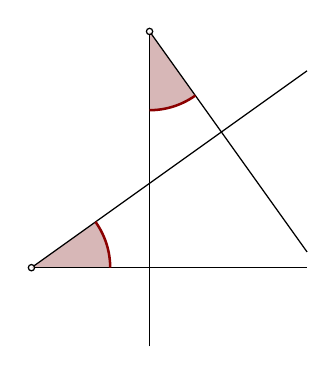
\begin{tikzpicture}
                        % \clip (0,0) rectangle (14.000000,10.000000);
                        {\footnotesize

                        % Changing color 215 183 183
                        \definecolor{r215g183b183}{rgb}{0.843137,0.717647,0.717647}%
                        \color{r215g183b183}% 

                        % Filling circle arc V D 35.54
                        \fill (1.500000,2.000000) -- (2.500000,2.000000) arc (0:35:1.000000 and 1.000000) -- (2.313733,2.581238) -- cycle;%

                        % Filling circle arc U E 35.54
                        \fill (3.000000,5.000000) -- (3.000000,4.000000) -- (3.000000,4.000000) arc (270:305:1.000000 and 1.000000) -- (3.581238,4.186266) -- cycle;%

                        % Changing color 0 0 0
                        \definecolor{r0g0b0}{rgb}{0.000000,0.000000,0.000000}%
                        \color{r0g0b0}% 

                        % Marking point V by circle
                        \draw [line width=0.016cm] (1.500000,2.000000) circle (0.040000);%

                        % Drawing line V A
                        % \draw [line width=0.016cm] (1.000000,2.000000) -- (1.460000,2.000000);%
                        \draw [line width=0.016cm] (1.540000,2.000000) -- (5.000000,2.000000);%

                        % Drawing line V B
                        % \draw [line width=0.016cm] (1.000000,1.642857) -- (1.467451,1.976750);%
                        \draw [line width=0.016cm] (1.532549,2.023250) -- (5.000000,4.500000);%

                        % Marking point U by circle
                        \draw [line width=0.016cm] (3.000000,5.000000) circle (0.040000);%

                        % Drawing line r
                        % \draw [line width=0.016cm] (2.642857,5.500000) -- (2.976750,5.032549);%
                        \draw [line width=0.016cm] (3.023250,4.967451) -- (5.000000,2.200000);%

                        % Drawing line s
                        \draw [line width=0.016cm] (3.000000,1.000000) -- (3.000000,4.960000);%
                        % \draw [line width=0.016cm] (3.000000,5.040000) -- (3.000000,5.500000);%

                        % Changing color 139 0 0
                        \definecolor{r139g0b0}{rgb}{0.545098,0.000000,0.000000}%
                        \color{r139g0b0}% 

                        % Drawing arc V D 35.54
                        \draw [line width=0.032cm] (2.500000,2.000000) arc (360:360:1.000000 and 1.000000) --(2.500000,2.000000) arc (0:35:1.000000 and 1.000000) -- (2.313733,2.581238);%

                        % Drawing arc U E 35.54
                        \draw [line width=0.032cm] (3.000000,4.000000) -- (3.000000,4.000000) arc (270:305:1.000000 and 1.000000) -- (3.581238,4.186266);%
                        \color{black}
                        }
                    \end{tikzpicture} ~~~~~~~~~~
                    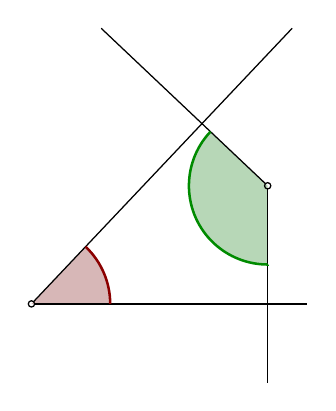
\begin{tikzpicture}
                        % \clip (0,0) rectangle (14.000000,10.000000);
                        {\footnotesize

                        % Changing color 215 183 183
                        \definecolor{r215g183b183}{rgb}{0.843137,0.717647,0.717647}%
                        \color{r215g183b183}% 

                        % Filling circle arc V D 46.59
                        \fill (1.500000,2.000000) -- (2.500000,2.000000) arc (0:46:1.000000 and 1.000000) -- (2.187200,2.726468) -- cycle;%

                        % Changing color 183 215 183
                        \definecolor{r183g215b183}{rgb}{0.717647,0.843137,0.717647}%
                        \color{r183g215b183}% 

                        % Filling circle arc U F 133.41
                        \fill (4.500000,3.500000) -- (3.773532,4.187200) -- (3.768646,4.181998) arc (137:270:1.000000 and 1.000000) -- (4.500000,2.500000) -- cycle;%

                        % Changing color 0 0 0
                        \definecolor{r0g0b0}{rgb}{0.000000,0.000000,0.000000}%
                        \color{r0g0b0}% 

                        % Marking point V by circle
                        \draw [line width=0.016cm] (1.500000,2.000000) circle (0.040000);%

                        % Drawing line V A
                        % \draw [line width=0.016cm] (1.000000,2.000000) -- (1.460000,2.000000);%
                        \draw [line width=0.016cm] (1.540000,2.000000) -- (5.000000,2.000000);%

                        % Drawing line V B
                        \draw [line width=0.016cm] (4.810811,5.500000) -- (1.527488,2.029059);%
                        % \draw [line width=0.016cm] (1.472512,1.970941) -- (1.000000,1.471429);%

                        % Marking point U by circle
                        \draw [line width=0.016cm] (4.500000,3.500000) circle (0.040000);%

                        % Drawing line r
                        \draw [line width=0.016cm] (2.385714,5.500000) -- (4.470941,3.527488);%
                        % \draw [line width=0.016cm] (4.529059,3.472512) -- (5.000000,3.027027);%

                        % Drawing line s
                        \draw [line width=0.016cm] (4.500000,1.000000) -- (4.500000,3.460000);%
                        % \draw [line width=0.016cm] (4.500000,3.540000) -- (4.500000,5.500000);%

                        % Changing color 139 0 0
                        \definecolor{r139g0b0}{rgb}{0.545098,0.000000,0.000000}%
                        \color{r139g0b0}% 

                        % Drawing arc V D 46.59
                        \draw [line width=0.032cm] (2.500000,2.000000) arc (360:360:1.000000 and 1.000000) --(2.500000,2.000000) arc (0:46:1.000000 and 1.000000) -- (2.187200,2.726468);%

                        % Changing color 0 139 0
                        \definecolor{r0g139b0}{rgb}{0.000000,0.545098,0.000000}%
                        \color{r0g139b0}% 

                        % Drawing arc U F 133.41
                        \draw [line width=0.032cm] (3.773532,4.187200) -- (3.768646,4.181998) arc (137:270:1.000000 and 1.000000) -- (4.500000,2.500000);%
                        \color{black}
                        }
                    \end{tikzpicture}

                \end{figure}
            \end{izrek}
        


            \begin{definicija}
                        \textbf{Pravokotna projekcija} točke $T$ na premico $p$ je točka $T'$, 
                        ki leži na presečišču premice $p$ in pravokotnice $q$ skozi točko $T$ na premico $p$. \\
                        Točka $T'$ je točki $T$ najbližja točka premice $p$. 
                    \end{definicija}
                    
                    
                        \textbf{Razdalja} točke $T$ od premice $p$ je: $$d(T,p)=d(T,T')=\left\lvert TT'\right\rvert.$$

                        

                    
                    \begin{figure}[H]
                        \begin{tikzpicture}
                            % \clip (0,0) rectangle (14.000000,10.000000);
                            {\footnotesize
                            
                            % Drawing line Q
                            \draw [line width=0.016cm] (3.000000,1.000000) -- (2.932918,1.134164);%
                            \draw [line width=0.016cm] (2.899377,1.201246) -- (2.832295,1.335410);%
                            \draw [line width=0.016cm] (2.798754,1.402492) -- (2.731672,1.536656);%
                            \draw [line width=0.016cm] (2.698131,1.603738) -- (2.631049,1.737902);%
                            \draw [line width=0.016cm] (2.582111,1.835777) -- (2.530426,1.939149);%
                            \draw [line width=0.016cm] (2.496885,2.006231) -- (2.429803,2.140395);%
                            \draw [line width=0.016cm] (2.396262,2.207477) -- (2.329180,2.341641);%
                            \draw [line width=0.016cm] (2.295639,2.408723) -- (2.228557,2.542887);%
                            \draw [line width=0.016cm] (2.195016,2.609969) -- (2.127933,2.744133);%
                            \draw [line width=0.016cm] (2.094392,2.811215) -- (2.027310,2.945379);%
                            \draw [line width=0.016cm] (1.993769,3.012461) -- (1.926687,3.146625);%
                            \draw [line width=0.016cm] (1.893146,3.213707) -- (1.826064,3.347871);%
                            \draw [line width=0.016cm] (1.792523,3.414953) -- (1.725441,3.549117);%
                            \draw [line width=0.016cm] (1.691900,3.616200) -- (1.624818,3.750364);%
                            \draw [line width=0.016cm] (1.591277,3.817446) -- (1.524195,3.951610);%
                            \draw [line width=0.016cm] (1.482111,4.035777) -- (1.423572,4.152856);%
                            \draw [line width=0.016cm] (1.390031,4.219938) -- (1.322949,4.354102);%
                            \draw [line width=0.016cm] (1.289408,4.421184) -- (1.250000,4.500000);%
                            
                            % Marking point q
                            \draw (1.847000,3.306000) node [anchor=east] { $q$ };%
                            
                            % Marking point T by circle
                            \draw [line width=0.016cm] (1.500000,4.000000) circle (0.040000);%
                            \draw (1.550000,4.000000) node [anchor=south] { $T$ };%
                            
                            % Marking point \frac{\pi}{2}
                            \draw (2.250000,2.000000) node  { $\frac{\pi}{2}$ };%
                            
                            % Changing color 0 0 255
                            \definecolor{r0g0b255}{rgb}{0.000000,0.000000,1.000000}%
                            \color{r0g0b255}% 
                            
                            % Drawing line P
                            \draw [line width=0.016cm] (1.000000,1.000000) -- (2.564223,1.782111);%
                            \draw [line width=0.016cm] (2.635777,1.817889) -- (4.500000,2.750000);%
                            
                            % Marking point p
                            \draw (4.155000,2.578000) node [anchor=north] { $p$ };%
                            
                            % Changing color 255 0 0
                            \definecolor{r255g0b0}{rgb}{1.000000,0.000000,0.000000}%
                            \color{r255g0b0}% 
                            
                            % Marking point T' by circle
                            \draw [line width=0.016cm] (2.600000,1.800000) circle (0.040000);%
                            \draw (2.500000,1.900000) node [anchor=south west] { $T'$ };%
                            \color{black}
                            }
                        \end{tikzpicture}
                    \end{figure}

                    
            
                Pravokotna projekcija daljice $AB$ na premico je daljica $A'B'$, katere krajišči sta pravokotni projekciji točk $A$ in $B$.

                
            % \note{
            %     TABLA: konstrukcija pravokotne projekcije točke  z ravnilom in šestilom
            %     \\
            %     TABLA: konstruckija pravokotne projekcije daljice z ravnilom in šestilom
            % }


        


        
        \subsection*{Toge preslikave}
            
            \begin{definicija}
                \textbf{Toga preslikava} (izometrija) je preslikava v ravnini, ki ohranja razdalje.
                \begin{align*}
                    \tau:~ &A \mapsto A' \\ 
                    \tau:~ &B \mapsto B' \\ 
                    d(A,B)&=d(A',B')
                \end{align*}
            \end{definicija}

            
                Med toge preslikave spadajo:
                    \begin{itemize}
                        \item \textbf{vzporedni premiki};
                        \item \textbf{zrcaljenje preko premice/premice};
                        \item \textbf{rotacija okoli točke}.
                    \end{itemize}

                Če kombiniramo več togih preslikav, je dobljena preslikava spet toga preslikava.

                
        


        

            
                \textbf{Vzporedni premik} ali \textbf{translacija} za dano usmerjeno daljico $\overrightarrow{MN}$ preslika točko $T$ v tako točko $T'$, da sta daljici $TT'$ in $MN$ enako dolgi, vzporedni in enako usmerjeni. \\  %(vektorja $\overrightarrow{TT'}$ in $\overrightarrow{AB}$ sta enaka). \\
                
                % \begin{figure}
                %     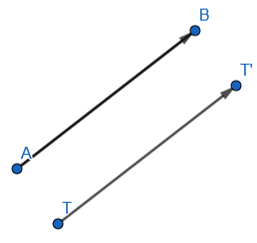
\includegraphics[scale=0.5]{Slike in skice/Vzporedni_premik_tocke.png}
                %     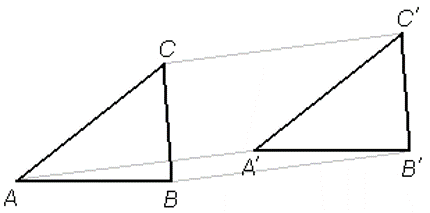
\includegraphics[scale=0.5]{Slike in skice/Vzporedni_premik_trikotnika.png}
                % \end{figure}

                \begin{figure}[H]
                    \begin{tikzpicture}
                        % \clip (0,0) rectangle (14.000000,10.000000);
                        {\footnotesize
                        
                        % Drawing segment M N
                        \draw [line width=0.016cm] (1.537947,2.512649) -- (4.462053,3.487351);%
                        
                        % Drawing arrow M N 1.00
                        \draw [line width=0.016cm] (4.205447,3.443092) -- (4.460726,3.492412);%
                        \draw [line width=0.016cm] (4.205447,3.443092) -- (4.405943,3.468648);%
                        \draw [line width=0.016cm] (4.230213,3.368795) -- (4.464028,3.482506);%
                        \draw [line width=0.016cm] (4.230213,3.368795) -- (4.405943,3.468648);%
                        
                        % Drawing segment T T'
                        \draw [line width=0.016cm] (2.037947,1.512649) -- (2.142302,1.547434);%
                        \draw [line width=0.016cm] (2.213454,1.571151) -- (2.355756,1.618585);%
                        \draw [line width=0.016cm] (2.426907,1.642302) -- (2.569210,1.689737);%
                        \draw [line width=0.016cm] (2.640361,1.713454) -- (2.782664,1.760888);%
                        \draw [line width=0.016cm] (2.853815,1.784605) -- (2.996117,1.832039);%
                        \draw [line width=0.016cm] (3.067269,1.855756) -- (3.209571,1.903190);%
                        \draw [line width=0.016cm] (3.280722,1.926907) -- (3.423025,1.974342);%
                        \draw [line width=0.016cm] (3.494176,1.998059) -- (3.636479,2.045493);%
                        \draw [line width=0.016cm] (3.707630,2.069210) -- (3.849932,2.116644);%
                        \draw [line width=0.016cm] (3.921084,2.140361) -- (4.063386,2.187795);%
                        \draw [line width=0.016cm] (4.134537,2.211512) -- (4.276840,2.258947);%
                        \draw [line width=0.016cm] (4.347991,2.282664) -- (4.490294,2.330098);%
                        \draw [line width=0.016cm] (4.561445,2.353815) -- (4.703747,2.401249);%
                        \draw [line width=0.016cm] (4.774899,2.424966) -- (4.917201,2.472400);%
                        
                        % Drawing arrow T T' 1.00
                        \draw [line width=0.016cm] (4.705447,2.443092) -- (4.960726,2.492412);%
                        \draw [line width=0.016cm] (4.705447,2.443092) -- (4.905943,2.468648);%
                        \draw [line width=0.016cm] (4.730213,2.368795) -- (4.964028,2.482506);%
                        \draw [line width=0.016cm] (4.730213,2.368795) -- (4.905943,2.468648);%
                        
                        % Marking point T by circle
                        \draw [line width=0.016cm] (2.000000,1.500000) circle (0.040000);%
                        \draw (2.000000,1.500000) node [anchor=north] { $T$ };%
                        
                        % Marking point A by circle
                        \draw [line width=0.016cm] (6.000000,2.000000) circle (0.040000);%
                        \draw (6.000000,2.000000) node [anchor=north] { $A$ };%
                        
                        % Marking point B by circle
                        \draw [line width=0.016cm] (9.000000,2.000000) circle (0.040000);%
                        \draw (9.000000,2.000000) node [anchor=north] { $B$ };%
                        
                        % Marking point C by circle
                        \draw [line width=0.016cm] (7.000000,4.000000) circle (0.040000);%
                        \draw (7.000000,4.000000) node [anchor=south] { $C$ };%
                        
                        % Drawing segment A B
                        \draw [line width=0.016cm] (6.040000,2.000000) -- (8.960000,2.000000);%
                        
                        % Drawing segment B C
                        \draw [line width=0.016cm] (8.971716,2.028284) -- (7.028284,3.971716);%
                        
                        % Drawing segment A C
                        \draw [line width=0.016cm] (6.017889,2.035777) -- (6.982111,3.964223);%
                        
                        % Drawing segment A' B'
                        \draw [line width=0.016cm] (9.040000,3.000000) -- (11.960000,3.000000);%
                        
                        % Drawing segment B' C'
                        \draw [line width=0.016cm] (11.971716,3.028284) -- (10.028284,4.971716);%
                        
                        % Drawing segment A' C'
                        \draw [line width=0.016cm] (9.017889,3.035777) -- (9.982111,4.964223);%
                        
                        % Drawing segment A A'
                        \draw [line width=0.016cm] (6.037947,2.012649) -- (6.142302,2.047434);%
                        \draw [line width=0.016cm] (6.213454,2.071151) -- (6.355756,2.118585);%
                        \draw [line width=0.016cm] (6.426907,2.142302) -- (6.569210,2.189737);%
                        \draw [line width=0.016cm] (6.640361,2.213454) -- (6.782664,2.260888);%
                        \draw [line width=0.016cm] (6.853815,2.284605) -- (6.996117,2.332039);%
                        \draw [line width=0.016cm] (7.067269,2.355756) -- (7.209571,2.403190);%
                        \draw [line width=0.016cm] (7.280722,2.426907) -- (7.423025,2.474342);%
                        \draw [line width=0.016cm] (7.494176,2.498059) -- (7.636479,2.545493);%
                        \draw [line width=0.016cm] (7.707630,2.569210) -- (7.849932,2.616644);%
                        \draw [line width=0.016cm] (7.921084,2.640361) -- (8.063386,2.687795);%
                        \draw [line width=0.016cm] (8.134537,2.711512) -- (8.276840,2.758947);%
                        \draw [line width=0.016cm] (8.347991,2.782664) -- (8.490294,2.830098);%
                        \draw [line width=0.016cm] (8.561445,2.853815) -- (8.703747,2.901249);%
                        \draw [line width=0.016cm] (8.774899,2.924966) -- (8.917201,2.972400);%
                        
                        % Drawing segment B B'
                        \draw [line width=0.016cm] (9.037947,2.012649) -- (9.142302,2.047434);%
                        \draw [line width=0.016cm] (9.213454,2.071151) -- (9.355756,2.118585);%
                        \draw [line width=0.016cm] (9.426907,2.142302) -- (9.569210,2.189737);%
                        \draw [line width=0.016cm] (9.640361,2.213454) -- (9.782664,2.260888);%
                        \draw [line width=0.016cm] (9.853815,2.284605) -- (9.996117,2.332039);%
                        \draw [line width=0.016cm] (10.067269,2.355756) -- (10.209571,2.403190);%
                        \draw [line width=0.016cm] (10.280722,2.426907) -- (10.423025,2.474342);%
                        \draw [line width=0.016cm] (10.494176,2.498059) -- (10.636479,2.545493);%
                        \draw [line width=0.016cm] (10.707630,2.569210) -- (10.849932,2.616644);%
                        \draw [line width=0.016cm] (10.921084,2.640361) -- (11.063386,2.687795);%
                        \draw [line width=0.016cm] (11.134537,2.711512) -- (11.276840,2.758947);%
                        \draw [line width=0.016cm] (11.347991,2.782664) -- (11.490294,2.830098);%
                        \draw [line width=0.016cm] (11.561445,2.853815) -- (11.703747,2.901249);%
                        \draw [line width=0.016cm] (11.774899,2.924966) -- (11.917201,2.972400);%
                        
                        % Drawing segment C C'
                        \draw [line width=0.016cm] (7.037947,4.012649) -- (7.142302,4.047434);%
                        \draw [line width=0.016cm] (7.213454,4.071151) -- (7.355756,4.118585);%
                        \draw [line width=0.016cm] (7.426907,4.142302) -- (7.569210,4.189737);%
                        \draw [line width=0.016cm] (7.640361,4.213454) -- (7.782664,4.260888);%
                        \draw [line width=0.016cm] (7.853815,4.284605) -- (7.996117,4.332039);%
                        \draw [line width=0.016cm] (8.067269,4.355756) -- (8.209571,4.403190);%
                        \draw [line width=0.016cm] (8.280722,4.426907) -- (8.423025,4.474342);%
                        \draw [line width=0.016cm] (8.494176,4.498059) -- (8.636479,4.545493);%
                        \draw [line width=0.016cm] (8.707630,4.569210) -- (8.849932,4.616644);%
                        \draw [line width=0.016cm] (8.921084,4.640361) -- (9.063386,4.687795);%
                        \draw [line width=0.016cm] (9.134537,4.711512) -- (9.276840,4.758947);%
                        \draw [line width=0.016cm] (9.347991,4.782664) -- (9.490294,4.830098);%
                        \draw [line width=0.016cm] (9.561445,4.853815) -- (9.703747,4.901249);%
                        \draw [line width=0.016cm] (9.774899,4.924966) -- (9.917201,4.972400);%
                        
                        % Changing color 0 0 255
                        \definecolor{r0g0b255}{rgb}{0.000000,0.000000,1.000000}%
                        \color{r0g0b255}% 
                        
                        % Marking point M by circle
                        \draw [line width=0.016cm] (1.500000,2.500000) circle (0.040000);%
                        \draw (1.500000,2.500000) node [anchor=north] { $M$ };%
                        
                        % Marking point N by circle
                        \draw [line width=0.016cm] (4.500000,3.500000) circle (0.040000);%
                        \draw (4.500000,3.500000) node [anchor=south] { $N$ };%
                        
                        % Changing color 255 0 0
                        \definecolor{r255g0b0}{rgb}{1.000000,0.000000,0.000000}%
                        \color{r255g0b0}% 
                        
                        % Marking point T' by circle
                        \draw [line width=0.016cm] (5.000000,2.500000) circle (0.040000);%
                        \draw (5.000000,2.500000) node [anchor=south] { $T'$ };%
                        
                        % Marking point C' by circle
                        \draw [line width=0.016cm] (10.000000,5.000000) circle (0.040000);%
                        \draw (10.000000,5.000000) node [anchor=south] { $C'$ };%
                        
                        % Marking point A' by circle
                        \draw [line width=0.016cm] (9.000000,3.000000) circle (0.040000);%
                        \draw (9.000000,3.000000) node [anchor=north] { $A'$ };%
                        
                        % Marking point B' by circle
                        \draw [line width=0.016cm] (12.000000,3.000000) circle (0.040000);%
                        \draw (12.000000,3.000000) node [anchor=north] { $B'$ };%
                        \color{black}
                        }
                    \end{tikzpicture}
                        
                \end{figure}

                
        
            Vzporedni premik ohranja orientacijo likov, daljice preslika v enako dolge vzporedne daljice, ohranja velikost kotov, like preslika v skladne like, nima negibnih točk za $\overrightarrow{MN}\neq \overrightarrow{0}$.

            

        



        % 
            
        %     Če smo kot  odmerili v smeri, ki je nasprotna smeri vrtenja urnega kazalca, smo točko $T$ zavrteli v \textbf{pozitivni smeri} za kot $\alpha$, sicer pa v \textbf{negativni smeri}. 
        %     Namesto smeri vrtenja lahko usmerimo kot: vrtenju v pozitivni smeri ustreza \textbf{pozitivni kot}, vrtenju v negativni smeri pa \textbf{negativni kot}. \\
        %     ~\\


        % 


        

            
                \textbf{Zrcaljenje čez premico} $p$ preslika točko $T$ v tako točko $T'$, da premica $p$ pod pravim kotom razpolavlja daljico $TT'$.
                
                % \begin{figure}
                %     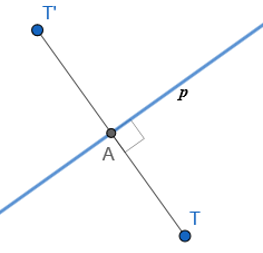
\includegraphics[scale=0.5]{Slike in skice/Zrcaljenje_tocke_cez_premico.png}
                %     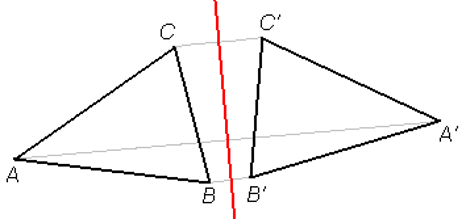
\includegraphics[scale=0.5]{Slike in skice/Zrcaljenje_lika_cez_premico.png}
                % \end{figure}

                \begin{figure}[H]
                    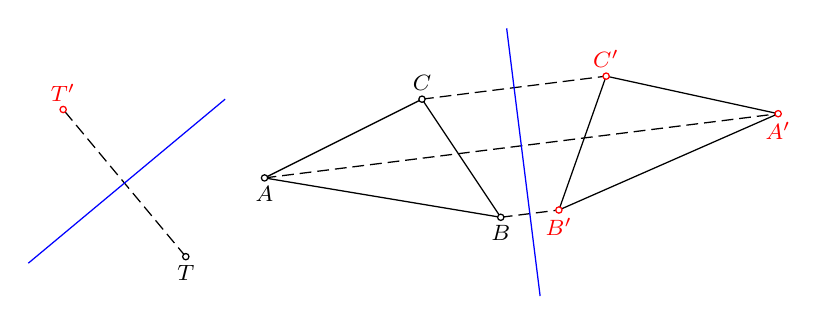
\begin{tikzpicture}
                        % \clip (0,0) rectangle (14.000000,10.000000);
                        {\footnotesize
                        
                        % Marking point T by circle
                        \draw [line width=0.016cm] (3.500000,1.500000) circle (0.040000);%
                        \draw (3.500000,1.500000) node [anchor=north] { $T$ };%
                        
                        % Drawing segment T T'
                        \draw [line width=0.016cm] (3.474393,1.530729) -- (3.403972,1.615233);%
                        \draw [line width=0.016cm] (3.355959,1.672850) -- (3.259931,1.788083);%
                        \draw [line width=0.016cm] (3.211917,1.845700) -- (3.115889,1.960933);%
                        \draw [line width=0.016cm] (3.067876,2.018549) -- (2.971848,2.133783);%
                        \draw [line width=0.016cm] (2.923834,2.191399) -- (2.827806,2.306632);%
                        \draw [line width=0.016cm] (2.779793,2.364249) -- (2.683765,2.479482);%
                        \draw [line width=0.016cm] (2.635751,2.537099) -- (2.539723,2.652332);%
                        \draw [line width=0.016cm] (2.491710,2.709949) -- (2.395682,2.825182);%
                        \draw [line width=0.016cm] (2.347668,2.882798) -- (2.251640,2.998031);%
                        \draw [line width=0.016cm] (2.203627,3.055648) -- (2.107599,3.170881);%
                        \draw [line width=0.016cm] (2.059585,3.228498) -- (1.968230,3.338124);%
                        
                        % Drawing segment C C'
                        \draw [line width=0.016cm] (6.539691,3.504961) -- (6.648842,3.518605);%
                        \draw [line width=0.016cm] (6.723263,3.527908) -- (6.872104,3.546513);%
                        \draw [line width=0.016cm] (6.946525,3.555816) -- (7.095367,3.574421);%
                        \draw [line width=0.016cm] (7.169788,3.583723) -- (7.318629,3.602329);%
                        \draw [line width=0.016cm] (7.393050,3.611631) -- (7.541892,3.630236);%
                        \draw [line width=0.016cm] (7.616313,3.639539) -- (7.765154,3.658144);%
                        \draw [line width=0.016cm] (7.839575,3.667447) -- (7.988417,3.686052);%
                        \draw [line width=0.016cm] (8.062838,3.695355) -- (8.211679,3.713960);%
                        \draw [line width=0.016cm] (8.286100,3.723263) -- (8.434942,3.741868);%
                        \draw [line width=0.016cm] (8.509363,3.751170) -- (8.658204,3.769776);%
                        \draw [line width=0.016cm] (8.732625,3.779078) -- (8.798770,3.787346);%
                        
                        % Drawing segment B B'
                        \draw [line width=0.016cm] (7.539691,2.004961) -- (7.648842,2.018605);%
                        \draw [line width=0.016cm] (7.723263,2.027908) -- (7.872104,2.046513);%
                        \draw [line width=0.016cm] (7.946525,2.055816) -- (8.095367,2.074421);%
                        \draw [line width=0.016cm] (8.169788,2.083723) -- (8.198770,2.087346);%
                        
                        % Drawing segment A A'
                        \draw [line width=0.016cm] (4.539691,2.504961) -- (4.648842,2.518605);%
                        \draw [line width=0.016cm] (4.723263,2.527908) -- (4.872104,2.546513);%
                        \draw [line width=0.016cm] (4.946525,2.555816) -- (5.095367,2.574421);%
                        \draw [line width=0.016cm] (5.169788,2.583723) -- (5.318629,2.602329);%
                        \draw [line width=0.016cm] (5.393050,2.611631) -- (5.541892,2.630236);%
                        \draw [line width=0.016cm] (5.616313,2.639539) -- (5.765154,2.658144);%
                        \draw [line width=0.016cm] (5.839575,2.667447) -- (5.988417,2.686052);%
                        \draw [line width=0.016cm] (6.062838,2.695355) -- (6.211679,2.713960);%
                        \draw [line width=0.016cm] (6.286100,2.723263) -- (6.434942,2.741868);%
                        \draw [line width=0.016cm] (6.509363,2.751170) -- (6.658204,2.769776);%
                        \draw [line width=0.016cm] (6.732625,2.779078) -- (6.881467,2.797683);%
                        \draw [line width=0.016cm] (6.955888,2.806986) -- (7.104729,2.825591);%
                        \draw [line width=0.016cm] (7.179150,2.834894) -- (7.327992,2.853499);%
                        \draw [line width=0.016cm] (7.402413,2.862802) -- (7.551254,2.881407);%
                        \draw [line width=0.016cm] (7.625675,2.890709) -- (7.774517,2.909315);%
                        \draw [line width=0.016cm] (7.848938,2.918617) -- (7.997780,2.937222);%
                        \draw [line width=0.016cm] (8.072200,2.946525) -- (8.221042,2.965130);%
                        \draw [line width=0.016cm] (8.295463,2.974433) -- (8.444305,2.993038);%
                        \draw [line width=0.016cm] (8.518725,3.002341) -- (8.667567,3.020946);%
                        \draw [line width=0.016cm] (8.741988,3.030248) -- (8.890830,3.048854);%
                        \draw [line width=0.016cm] (8.965250,3.058156) -- (9.114092,3.076762);%
                        \draw [line width=0.016cm] (9.188513,3.086064) -- (9.337355,3.104669);%
                        \draw [line width=0.016cm] (9.411775,3.113972) -- (9.560617,3.132577);%
                        \draw [line width=0.016cm] (9.635038,3.141880) -- (9.783880,3.160485);%
                        \draw [line width=0.016cm] (9.858301,3.169788) -- (10.007142,3.188393);%
                        \draw [line width=0.016cm] (10.081563,3.197695) -- (10.230405,3.216301);%
                        \draw [line width=0.016cm] (10.304826,3.225603) -- (10.453667,3.244208);%
                        \draw [line width=0.016cm] (10.528088,3.253511) -- (10.676930,3.272116);%
                        \draw [line width=0.016cm] (10.751351,3.281419) -- (10.900192,3.300024);%
                        \draw [line width=0.016cm] (10.974613,3.309327) -- (10.983386,3.310423);%
                        
                        % Marking point C by circle
                        \draw [line width=0.016cm] (6.500000,3.500000) circle (0.040000);%
                        \draw (6.500000,3.500000) node [anchor=south] { $C$ };%
                        
                        % Marking point A by circle
                        \draw [line width=0.016cm] (4.500000,2.500000) circle (0.040000);%
                        \draw (4.500000,2.500000) node [anchor=north] { $A$ };%
                        
                        % Marking point B by circle
                        \draw [line width=0.016cm] (7.500000,2.000000) circle (0.040000);%
                        \draw (7.500000,2.000000) node [anchor=north] { $B$ };%
                        
                        % Drawing segment A B
                        \draw [line width=0.016cm] (4.539456,2.493424) -- (7.460544,2.006576);%
                        
                        % Drawing segment B C
                        \draw [line width=0.016cm] (7.477812,2.033282) -- (6.522188,3.466718);%
                        
                        % Drawing segment C A
                        \draw [line width=0.016cm] (6.464223,3.482111) -- (4.535777,2.517889);%
                        
                        % Drawing segment C' A'
                        \draw [line width=0.016cm] (8.877541,3.783776) -- (10.983997,3.323916);%
                        
                        % Drawing segment B' C'
                        \draw [line width=0.016cm] (8.251774,2.130027) -- (8.825149,3.754588);%
                        
                        % Drawing segment A' B'
                        \draw [line width=0.016cm] (10.986454,3.299299) -- (8.275085,2.108394);%
                        
                        % Changing color 0 0 255
                        \definecolor{r0g0b255}{rgb}{0.000000,0.000000,1.000000}%
                        \color{r0g0b255}% 
                        
                        % Drawing segment X Y
                        \draw [line width=0.016cm] (4.000000,3.500000) -- (1.500000,1.416667);%
                        
                        % Drawing line r
                        \draw [line width=0.016cm] (8.000000,1.000000) -- (7.575000,4.400000);%
                        
                        % Changing color 255 0 0
                        \definecolor{r255g0b0}{rgb}{1.000000,0.000000,0.000000}%
                        \color{r255g0b0}% 
                        
                        % Marking point T' by circle
                        \draw [line width=0.016cm] (1.942623,3.368852) circle (0.040000);%
                        \draw (1.942623,3.368852) node [anchor=south] { $T'$ };%
                        
                        % Marking point C' by circle
                        \draw [line width=0.016cm] (8.838462,3.792308) circle (0.040000);%
                        \draw (8.838462,3.792308) node [anchor=south] { $C'$ };%
                        
                        % Marking point B' by circle
                        \draw [line width=0.016cm] (8.238462,2.092308) circle (0.040000);%
                        \draw (8.238462,2.092308) node [anchor=north] { $B'$ };%
                        
                        % Marking point A' by circle
                        \draw [line width=0.016cm] (11.023077,3.315385) circle (0.040000);%
                        \draw (11.023077,3.315385) node [anchor=north] { $A'$ };%
                        \color{black}
                        }
                    \end{tikzpicture}
                        
                \end{figure}

                
                Zrcaljenje čez premico daljice preslika v enako dolge daljice, ohranja velikost kotov, ne ohranja orientacije likov, like preslika v skladne like, premic ne preslika v vzporedne premice.

                
            % \note{
            %     TABLA: konstrukcija zracljenja točke, daljice in trikotnika preko premice
            %     \\
            %     S pomočjo skic na tabli/okviru ugotavljanje lastnosti zrcaljenja preko premice.
            %     \\
            %     TABLA: Primer enakokrakega trikotnika (osnovnica AC) s simetralo kota z vrhom v C, ki seka c v N. (Dokaz skladnosti trikotnikov ANC in BNC.)
            % }
        

        
        

            
                \textbf{Zrcaljenje čez točko} $O$ preslika točko $T$ v tako točko $T'$, da je $O$ razpolovišče daljice $TT'$. Ta preslikava je enaka vrtenju okrog točke za $180^\circ$.

                % \begin{figure}
                %     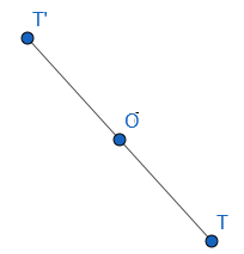
\includegraphics[scale=0.5]{Slike in skice/Zrcaljenje_tocke_cez_tocko.png}
                %     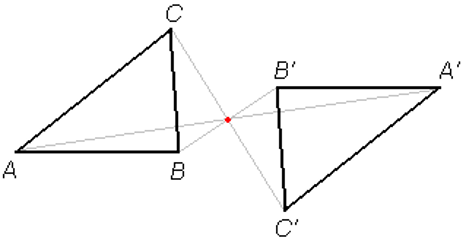
\includegraphics[scale=0.5]{Slike in skice/Zrcaljenje_lika_cez_tocko.png}
                % \end{figure}

                \begin{figure}[H]
                    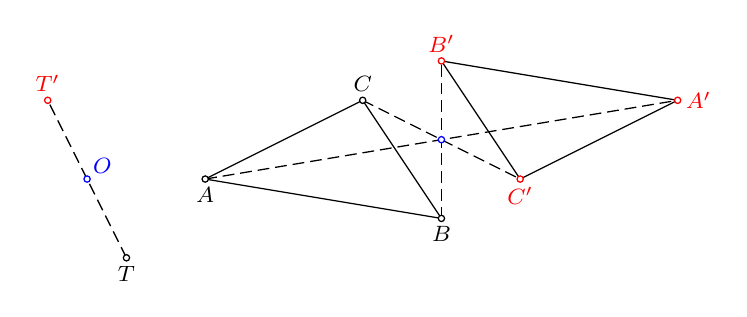
\begin{tikzpicture}
                        % \clip (0,0) rectangle (14.000000,10.000000);
                        {\footnotesize
                        
                        % Marking point T by circle
                        \draw [line width=0.016cm] (3.500000,1.500000) circle (0.040000);%
                        \draw (3.500000,1.500000) node [anchor=north] { $T$ };%
                        
                        % Drawing segment T T'
                        \draw [line width=0.016cm] (3.482111,1.535777) -- (3.432918,1.634164);%
                        \draw [line width=0.016cm] (3.399377,1.701246) -- (3.332295,1.835410);%
                        \draw [line width=0.016cm] (3.298754,1.902492) -- (3.231672,2.036656);%
                        \draw [line width=0.016cm] (3.198131,2.103738) -- (3.131049,2.237902);%
                        \draw [line width=0.016cm] (3.097508,2.304984) -- (3.030426,2.439149);%
                        \draw [line width=0.016cm] (2.982111,2.535777) -- (2.929803,2.640395);%
                        \draw [line width=0.016cm] (2.896262,2.707477) -- (2.829180,2.841641);%
                        \draw [line width=0.016cm] (2.795639,2.908723) -- (2.728557,3.042887);%
                        \draw [line width=0.016cm] (2.695016,3.109969) -- (2.627933,3.244133);%
                        \draw [line width=0.016cm] (2.594392,3.311215) -- (2.527310,3.445379);%
                        
                        % Drawing segment C C'
                        \draw [line width=0.016cm] (6.535777,3.482111) -- (6.634164,3.432918);%
                        \draw [line width=0.016cm] (6.701246,3.399377) -- (6.835410,3.332295);%
                        \draw [line width=0.016cm] (6.902492,3.298754) -- (7.036656,3.231672);%
                        \draw [line width=0.016cm] (7.103738,3.198131) -- (7.237902,3.131049);%
                        \draw [line width=0.016cm] (7.304984,3.097508) -- (7.439149,3.030426);%
                        \draw [line width=0.016cm] (7.535777,2.982111) -- (7.640395,2.929803);%
                        \draw [line width=0.016cm] (7.707477,2.896262) -- (7.841641,2.829180);%
                        \draw [line width=0.016cm] (7.908723,2.795639) -- (8.042887,2.728557);%
                        \draw [line width=0.016cm] (8.109969,2.695016) -- (8.244133,2.627933);%
                        \draw [line width=0.016cm] (8.311215,2.594392) -- (8.445379,2.527310);%
                        
                        % Drawing segment B B'
                        \draw [line width=0.016cm] (7.500000,2.040000) -- (7.500000,2.150000);%
                        \draw [line width=0.016cm] (7.500000,2.225000) -- (7.500000,2.375000);%
                        \draw [line width=0.016cm] (7.500000,2.450000) -- (7.500000,2.600000);%
                        \draw [line width=0.016cm] (7.500000,2.675000) -- (7.500000,2.825000);%
                        \draw [line width=0.016cm] (7.500000,2.900000) -- (7.500000,2.960000);%
                        \draw [line width=0.016cm] (7.500000,3.040000) -- (7.500000,3.050000);%
                        \draw [line width=0.016cm] (7.500000,3.125000) -- (7.500000,3.275000);%
                        \draw [line width=0.016cm] (7.500000,3.350000) -- (7.500000,3.500000);%
                        \draw [line width=0.016cm] (7.500000,3.575000) -- (7.500000,3.725000);%
                        \draw [line width=0.016cm] (7.500000,3.800000) -- (7.500000,3.950000);%
                        
                        % Drawing segment A A'
                        \draw [line width=0.016cm] (4.539456,2.506576) -- (4.647959,2.524660);%
                        \draw [line width=0.016cm] (4.721939,2.536990) -- (4.869898,2.561650);%
                        \draw [line width=0.016cm] (4.943877,2.573980) -- (5.091836,2.598639);%
                        \draw [line width=0.016cm] (5.165816,2.610969) -- (5.313775,2.635629);%
                        \draw [line width=0.016cm] (5.387755,2.647959) -- (5.535714,2.672619);%
                        \draw [line width=0.016cm] (5.609693,2.684949) -- (5.757652,2.709609);%
                        \draw [line width=0.016cm] (5.831632,2.721939) -- (5.979591,2.746598);%
                        \draw [line width=0.016cm] (6.053570,2.758928) -- (6.201530,2.783588);%
                        \draw [line width=0.016cm] (6.275509,2.795918) -- (6.423468,2.820578);%
                        \draw [line width=0.016cm] (6.497448,2.832908) -- (6.645407,2.857568);%
                        \draw [line width=0.016cm] (6.719386,2.869898) -- (6.867345,2.894558);%
                        \draw [line width=0.016cm] (6.941325,2.906887) -- (7.089284,2.931547);%
                        \draw [line width=0.016cm] (7.163264,2.943877) -- (7.311223,2.968537);%
                        \draw [line width=0.016cm] (7.385202,2.980867) -- (7.460544,2.993424);%
                        \draw [line width=0.016cm] (7.607141,3.017857) -- (7.755100,3.042517);%
                        \draw [line width=0.016cm] (7.829079,3.054847) -- (7.977039,3.079506);%
                        \draw [line width=0.016cm] (8.051018,3.091836) -- (8.198977,3.116496);%
                        \draw [line width=0.016cm] (8.272957,3.128826) -- (8.420916,3.153486);%
                        \draw [line width=0.016cm] (8.494895,3.165816) -- (8.642854,3.190476);%
                        \draw [line width=0.016cm] (8.716834,3.202806) -- (8.864793,3.227466);%
                        \draw [line width=0.016cm] (8.938773,3.239795) -- (9.086732,3.264455);%
                        \draw [line width=0.016cm] (9.160711,3.276785) -- (9.308670,3.301445);%
                        \draw [line width=0.016cm] (9.382650,3.313775) -- (9.530609,3.338435);%
                        \draw [line width=0.016cm] (9.604589,3.350765) -- (9.752548,3.375425);%
                        \draw [line width=0.016cm] (9.826527,3.387755) -- (9.974486,3.412414);%
                        \draw [line width=0.016cm] (10.048466,3.424744) -- (10.196425,3.449404);%
                        \draw [line width=0.016cm] (10.270404,3.461734) -- (10.418364,3.486394);%
                        
                        % Marking point C by circle
                        \draw [line width=0.016cm] (6.500000,3.500000) circle (0.040000);%
                        \draw (6.500000,3.500000) node [anchor=south] { $C$ };%
                        
                        % Marking point A by circle
                        \draw [line width=0.016cm] (4.500000,2.500000) circle (0.040000);%
                        \draw (4.500000,2.500000) node [anchor=north] { $A$ };%
                        
                        % Marking point B by circle
                        \draw [line width=0.016cm] (7.500000,2.000000) circle (0.040000);%
                        \draw (7.500000,2.000000) node [anchor=north] { $B$ };%
                        
                        % Drawing segment A B
                        \draw [line width=0.016cm] (4.539456,2.493424) -- (7.460544,2.006576);%
                        
                        % Drawing segment B C
                        \draw [line width=0.016cm] (7.477812,2.033282) -- (6.522188,3.466718);%
                        
                        % Drawing segment C A
                        \draw [line width=0.016cm] (6.464223,3.482111) -- (4.535777,2.517889);%
                        
                        % Drawing segment C' A'
                        \draw [line width=0.016cm] (8.535777,2.517889) -- (10.464223,3.482111);%
                        
                        % Drawing segment B' C'
                        \draw [line width=0.016cm] (7.522188,3.966718) -- (8.477812,2.533282);%
                        
                        % Drawing segment A' B'
                        \draw [line width=0.016cm] (10.460544,3.506576) -- (7.539456,3.993424);%
                        
                        % Changing color 0 0 255
                        \definecolor{r0g0b255}{rgb}{0.000000,0.000000,1.000000}%
                        \color{r0g0b255}% 
                        
                        % Marking point O by circle
                        \draw [line width=0.016cm] (3.000000,2.500000) circle (0.040000);%
                        \draw (2.970000,2.470000) node [anchor=south west] { $O$ };%
                        
                        % Marking point r by circle
                        \draw [line width=0.016cm] (7.500000,3.000000) circle (0.040000);%
                        
                        % Changing color 255 0 0
                        \definecolor{r255g0b0}{rgb}{1.000000,0.000000,0.000000}%
                        \color{r255g0b0}% 
                        
                        % Marking point T' by circle
                        \draw [line width=0.016cm] (2.500000,3.500000) circle (0.040000);%
                        \draw (2.500000,3.500000) node [anchor=south] { $T'$ };%
                        
                        % Marking point C' by circle
                        \draw [line width=0.016cm] (8.500000,2.500000) circle (0.040000);%
                        \draw (8.500000,2.500000) node [anchor=north] { $C'$ };%
                        
                        % Marking point B' by circle
                        \draw [line width=0.016cm] (7.500000,4.000000) circle (0.040000);%
                        \draw (7.500000,4.000000) node [anchor=south] { $B'$ };%
                        
                        % Marking point A' by circle
                        \draw [line width=0.016cm] (10.500000,3.500000) circle (0.040000);%
                        \draw (10.500000,3.500000) node [anchor=west] { $A'$ };%
                        \color{black}
                        }
                    \end{tikzpicture}
                        
                \end{figure}

                

            
                Zrcaljenje čez točko daljice preslika v enako dolge daljice, ohranja velikosti kotov in orientacijo likov, like preslika v skladne like, premice preslika v vzporedne premice.

                
            % \note{
            %     TABLA: konstrukcija zracljenja točke in trikotnika preko točke
            %     \\
            %     S pomočjo skic na tabli/okviru ugotavljanje lastnosti zrcaljenja preko točke.
            % }
        



        

            
                \textbf{Vrtenje} ali \textbf{zasuk} oziroma \textbf{rotacija} za kot $\varphi$ okrog točke $O$ preslika točko $T$ v točko $T'$, da velja: $\left\lvert OT\right\rvert = \left\lvert OT'\right\rvert$  in $\angle TOT' = \varphi$.

                % \begin{figure}
                %     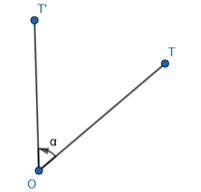
\includegraphics[scale=0.6]{Slike in skice/Rotacija tocke_okoli_tocke.png}
                %     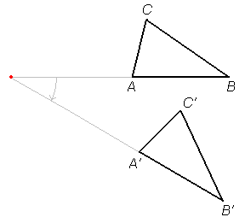
\includegraphics[scale=0.6]{Slike in skice/Rotacija_lika_okoli_tocke.png}
                % \end{figure}

                \begin{figure}[H]
                    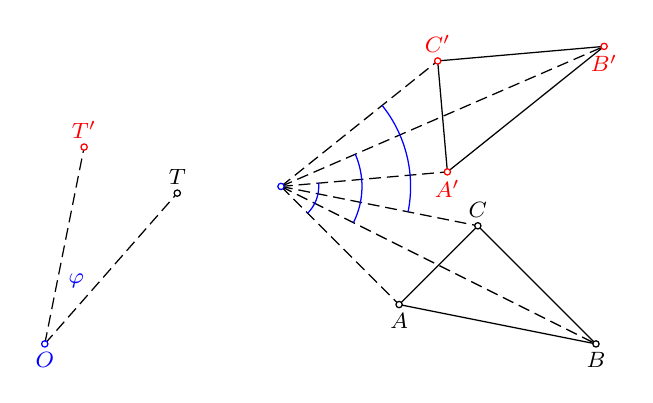
\begin{tikzpicture}
                        % \clip (0,0) rectangle (14.000000,10.000000);
                        {\footnotesize
                        
                        % Drawing segment O T
                        \draw [line width=0.016cm] (1.526405,1.530046) -- (1.599020,1.612672);%
                        \draw [line width=0.016cm] (1.648530,1.669009) -- (1.747550,1.781681);%
                        \draw [line width=0.016cm] (1.797059,1.838017) -- (1.896079,1.950690);%
                        \draw [line width=0.016cm] (1.945589,2.007026) -- (2.044609,2.119698);%
                        \draw [line width=0.016cm] (2.094119,2.176035) -- (2.193139,2.288707);%
                        \draw [line width=0.016cm] (2.242649,2.345043) -- (2.341668,2.457716);%
                        \draw [line width=0.016cm] (2.391178,2.514052) -- (2.490198,2.626724);%
                        \draw [line width=0.016cm] (2.539708,2.683060) -- (2.638728,2.795733);%
                        \draw [line width=0.016cm] (2.688238,2.852069) -- (2.787258,2.964742);%
                        \draw [line width=0.016cm] (2.836768,3.021078) -- (2.935787,3.133750);%
                        \draw [line width=0.016cm] (2.985297,3.190086) -- (3.084317,3.302759);%
                        \draw [line width=0.016cm] (3.133827,3.359095) -- (3.156608,3.385017);%
                        
                        % Drawing segment O T'
                        \draw [line width=0.016cm] (1.507845,1.539223) -- (1.529417,1.647087);%
                        \draw [line width=0.016cm] (1.544126,1.720631) -- (1.573544,1.867718);%
                        \draw [line width=0.016cm] (1.588252,1.941261) -- (1.617670,2.088348);%
                        \draw [line width=0.016cm] (1.632378,2.161892) -- (1.661796,2.308979);%
                        \draw [line width=0.016cm] (1.676505,2.382523) -- (1.705922,2.529610);%
                        \draw [line width=0.016cm] (1.720631,2.603153) -- (1.750048,2.750240);%
                        \draw [line width=0.016cm] (1.764757,2.823784) -- (1.794174,2.970871);%
                        \draw [line width=0.016cm] (1.808883,3.044415) -- (1.838300,3.191502);%
                        \draw [line width=0.016cm] (1.853009,3.265045) -- (1.882426,3.412132);%
                        \draw [line width=0.016cm] (1.897135,3.485676) -- (1.926553,3.632763);%
                        \draw [line width=0.016cm] (1.941261,3.706307) -- (1.970679,3.853394);%
                        \draw [line width=0.016cm] (1.985387,3.926937) -- (1.992155,3.960777);%
                        
                        % Marking point C by circle
                        \draw [line width=0.016cm] (7.000000,3.000000) circle (0.040000);%
                        \draw (7.000000,3.000000) node [anchor=south] { $C$ };%
                        
                        % Marking point A by circle
                        \draw [line width=0.016cm] (6.000000,2.000000) circle (0.040000);%
                        \draw (6.000000,2.000000) node [anchor=north] { $A$ };%
                        
                        % Marking point B by circle
                        \draw [line width=0.016cm] (8.500000,1.500000) circle (0.040000);%
                        \draw (8.500000,1.500000) node [anchor=north] { $B$ };%
                        
                        % Drawing segment A B
                        \draw [line width=0.016cm] (6.039223,1.992155) -- (8.460777,1.507845);%
                        
                        % Drawing segment B C
                        \draw [line width=0.016cm] (8.471716,1.528284) -- (7.028284,2.971716);%
                        
                        % Drawing segment A C
                        \draw [line width=0.016cm] (6.028284,2.028284) -- (6.971716,2.971716);%
                        
                        % Drawing segment X A
                        \draw [line width=0.016cm] (4.528284,3.471716) -- (4.606066,3.393934);%
                        \draw [line width=0.016cm] (4.659099,3.340901) -- (4.765165,3.234835);%
                        \draw [line width=0.016cm] (4.818198,3.181802) -- (4.924264,3.075736);%
                        \draw [line width=0.016cm] (4.977297,3.022703) -- (5.083363,2.916637);%
                        \draw [line width=0.016cm] (5.136396,2.863604) -- (5.242462,2.757538);%
                        \draw [line width=0.016cm] (5.295495,2.704505) -- (5.401561,2.598439);%
                        \draw [line width=0.016cm] (5.454594,2.545406) -- (5.560660,2.439340);%
                        \draw [line width=0.016cm] (5.613693,2.386307) -- (5.719759,2.280241);%
                        \draw [line width=0.016cm] (5.772792,2.227208) -- (5.878858,2.121142);%
                        \draw [line width=0.016cm] (5.931891,2.068109) -- (5.971716,2.028284);%
                        
                        % Drawing segment X B
                        \draw [line width=0.016cm] (4.535777,3.482111) -- (4.634164,3.432918);%
                        \draw [line width=0.016cm] (4.701246,3.399377) -- (4.835410,3.332295);%
                        \draw [line width=0.016cm] (4.902492,3.298754) -- (5.036656,3.231672);%
                        \draw [line width=0.016cm] (5.103738,3.198131) -- (5.237902,3.131049);%
                        \draw [line width=0.016cm] (5.304984,3.097508) -- (5.439149,3.030426);%
                        \draw [line width=0.016cm] (5.506231,2.996885) -- (5.640395,2.929803);%
                        \draw [line width=0.016cm] (5.707477,2.896262) -- (5.841641,2.829180);%
                        \draw [line width=0.016cm] (5.908723,2.795639) -- (6.042887,2.728557);%
                        \draw [line width=0.016cm] (6.109969,2.695016) -- (6.244133,2.627933);%
                        \draw [line width=0.016cm] (6.311215,2.594392) -- (6.445379,2.527310);%
                        \draw [line width=0.016cm] (6.512461,2.493769) -- (6.646625,2.426687);%
                        \draw [line width=0.016cm] (6.713707,2.393146) -- (6.847871,2.326064);%
                        \draw [line width=0.016cm] (6.914953,2.292523) -- (7.049117,2.225441);%
                        \draw [line width=0.016cm] (7.116200,2.191900) -- (7.250364,2.124818);%
                        \draw [line width=0.016cm] (7.317446,2.091277) -- (7.451610,2.024195);%
                        \draw [line width=0.016cm] (7.518692,1.990654) -- (7.652856,1.923572);%
                        \draw [line width=0.016cm] (7.719938,1.890031) -- (7.854102,1.822949);%
                        \draw [line width=0.016cm] (7.921184,1.789408) -- (8.055348,1.722326);%
                        \draw [line width=0.016cm] (8.122430,1.688785) -- (8.256594,1.621703);%
                        \draw [line width=0.016cm] (8.323676,1.588162) -- (8.457840,1.521080);%
                        
                        % Drawing segment X C
                        \draw [line width=0.016cm] (4.539223,3.492155) -- (4.647087,3.470583);%
                        \draw [line width=0.016cm] (4.720631,3.455874) -- (4.867718,3.426456);%
                        \draw [line width=0.016cm] (4.941261,3.411748) -- (5.088348,3.382330);%
                        \draw [line width=0.016cm] (5.161892,3.367622) -- (5.308979,3.338204);%
                        \draw [line width=0.016cm] (5.382523,3.323495) -- (5.529610,3.294078);%
                        \draw [line width=0.016cm] (5.603153,3.279369) -- (5.750240,3.249952);%
                        \draw [line width=0.016cm] (5.823784,3.235243) -- (5.970871,3.205826);%
                        \draw [line width=0.016cm] (6.044415,3.191117) -- (6.191502,3.161700);%
                        \draw [line width=0.016cm] (6.265045,3.146991) -- (6.412132,3.117574);%
                        \draw [line width=0.016cm] (6.485676,3.102865) -- (6.632763,3.073447);%
                        \draw [line width=0.016cm] (6.706307,3.058739) -- (6.853394,3.029321);%
                        \draw [line width=0.016cm] (6.926937,3.014613) -- (6.960777,3.007845);%
                        
                        % Drawing segment A' B'
                        \draw [line width=0.016cm] (6.644470,3.709889) -- (8.572018,5.253598);%
                        
                        % Drawing segment B' C'
                        \draw [line width=0.016cm] (8.563392,5.275116) -- (6.529839,5.097203);%
                        
                        % Drawing segment A' C'
                        \draw [line width=0.016cm] (6.609762,3.724733) -- (6.493478,5.053869);%
                        
                        % Drawing segment X A'
                        \draw [line width=0.016cm] (4.539848,3.503486) -- (4.649429,3.513073);%
                        \draw [line width=0.016cm] (4.724144,3.519610) -- (4.873573,3.532683);%
                        \draw [line width=0.016cm] (4.948288,3.539220) -- (5.097717,3.552293);%
                        \draw [line width=0.016cm] (5.172431,3.558830) -- (5.321861,3.571903);%
                        \draw [line width=0.016cm] (5.396575,3.578440) -- (5.546004,3.591513);%
                        \draw [line width=0.016cm] (5.620719,3.598050) -- (5.770148,3.611124);%
                        \draw [line width=0.016cm] (5.844863,3.617660) -- (5.994292,3.630734);%
                        \draw [line width=0.016cm] (6.069007,3.637270) -- (6.218436,3.650344);%
                        \draw [line width=0.016cm] (6.293150,3.656880) -- (6.442580,3.669954);%
                        \draw [line width=0.016cm] (6.517294,3.676490) -- (6.573400,3.681399);%
                        
                        % Drawing segment X B'
                        \draw [line width=0.016cm] (4.536700,3.515908) -- (4.637627,3.559656);%
                        \draw [line width=0.016cm] (4.706440,3.589484) -- (4.844067,3.649140);%
                        \draw [line width=0.016cm] (4.912881,3.678968) -- (5.050507,3.738625);%
                        \draw [line width=0.016cm] (5.119321,3.768453) -- (5.256948,3.828109);%
                        \draw [line width=0.016cm] (5.325761,3.857937) -- (5.463388,3.917593);%
                        \draw [line width=0.016cm] (5.532201,3.947421) -- (5.669828,4.007077);%
                        \draw [line width=0.016cm] (5.738642,4.036905) -- (5.876268,4.096561);%
                        \draw [line width=0.016cm] (5.945082,4.126389) -- (6.082709,4.186046);%
                        \draw [line width=0.016cm] (6.151522,4.215874) -- (6.289149,4.275530);%
                        \draw [line width=0.016cm] (6.357962,4.305358) -- (6.495589,4.365014);%
                        \draw [line width=0.016cm] (6.564403,4.394842) -- (6.702029,4.454498);%
                        \draw [line width=0.016cm] (6.770843,4.484326) -- (6.908470,4.543982);%
                        \draw [line width=0.016cm] (6.977283,4.573810) -- (7.114910,4.633467);%
                        \draw [line width=0.016cm] (7.183723,4.663295) -- (7.321350,4.722951);%
                        \draw [line width=0.016cm] (7.390164,4.752779) -- (7.527790,4.812435);%
                        \draw [line width=0.016cm] (7.596604,4.842263) -- (7.734231,4.901919);%
                        \draw [line width=0.016cm] (7.803044,4.931747) -- (7.940671,4.991403);%
                        \draw [line width=0.016cm] (8.009484,5.021232) -- (8.147111,5.080888);%
                        \draw [line width=0.016cm] (8.215925,5.110716) -- (8.353551,5.170372);%
                        \draw [line width=0.016cm] (8.422365,5.200200) -- (8.559992,5.259856);%
                        
                        % Drawing segment X C'
                        \draw [line width=0.016cm] (4.531222,3.525004) -- (4.617081,3.593766);%
                        \draw [line width=0.016cm] (4.675621,3.640649) -- (4.792702,3.734415);%
                        \draw [line width=0.016cm] (4.851242,3.781298) -- (4.968323,3.875064);%
                        \draw [line width=0.016cm] (5.026864,3.921947) -- (5.143945,4.015714);%
                        \draw [line width=0.016cm] (5.202485,4.062597) -- (5.319566,4.156363);%
                        \draw [line width=0.016cm] (5.378106,4.203246) -- (5.495187,4.297012);%
                        \draw [line width=0.016cm] (5.553727,4.343895) -- (5.670808,4.437661);%
                        \draw [line width=0.016cm] (5.729349,4.484544) -- (5.846429,4.578310);%
                        \draw [line width=0.016cm] (5.904970,4.625193) -- (6.022051,4.718959);%
                        \draw [line width=0.016cm] (6.080591,4.765842) -- (6.197672,4.859608);%
                        \draw [line width=0.016cm] (6.256212,4.906491) -- (6.373293,5.000258);%
                        \draw [line width=0.016cm] (6.431834,5.047141) -- (6.458770,5.068713);%
                        
                        % Marking point T by circle
                        \draw [line width=0.016cm] (3.183013,3.415063) circle (0.040000);%
                        \draw (3.183013,3.415063) node [anchor=south] { $T$ };%
                        
                        % Changing color 0 0 255
                        \definecolor{r0g0b255}{rgb}{0.000000,0.000000,1.000000}%
                        \color{r0g0b255}% 
                        
                        % Marking point O by circle
                        \draw [line width=0.016cm] (1.500000,1.500000) circle (0.040000);%
                        \draw (1.500000,1.500000) node [anchor=north] { $O$ };%
                        
                        % Marking point \alpha
                        \draw (1.900000,2.300000) node  { $\varphi$ };%
                        
                        % Marking point X by circle
                        \draw [line width=0.016cm] (4.500000,3.500000) circle (0.040000);%
                        
                        % Drawing arc X a 50.00
                        \draw [line width=0.016cm] (4.839000,3.161000) -- (4.839000,3.161000) arc (315:360:0.479418 and 0.479418) --(4.979418,3.500000) arc (0:4:0.479418 and 0.479418) -- (4.977594,3.541784);%
                        
                        % Drawing arc X b 50.00
                        \draw [line width=0.016cm] (5.420000,3.040000) -- (5.424492,3.049095) arc (334:360:1.028591 and 1.028591) --(5.528591,3.500000) arc (0:23:1.028591 and 1.028591) -- (5.443745,3.909079);%
                        
                        % Drawing arc X c 50.00
                        \draw [line width=0.016cm] (6.114000,3.177000) -- (6.115761,3.185927) arc (349:360:1.646003 and 1.646003) --(6.146003,3.500000) arc (0:38:1.646003 and 1.646003) -- (5.784892,4.528775);%
                        
                        % Changing color 255 0 0
                        \definecolor{r255g0b0}{rgb}{1.000000,0.000000,0.000000}%
                        \color{r255g0b0}% 
                        
                        % Marking point T' by circle
                        \draw [line width=0.016cm] (2.000000,4.000000) circle (0.040000);%
                        \draw (2.000000,4.000000) node [anchor=south] { $T'$ };%
                        
                        % Marking point A' by circle
                        \draw [line width=0.016cm] (6.613248,3.684885) circle (0.040000);%
                        \draw (6.613248,3.684885) node [anchor=north] { $A'$ };%
                        
                        % Marking point B' by circle
                        \draw [line width=0.016cm] (8.603239,5.278602) circle (0.040000);%
                        \draw (8.603239,5.278602) node [anchor=north] { $B'$ };%
                        
                        % Marking point C' by circle
                        \draw [line width=0.016cm] (6.489991,5.093717) circle (0.040000);%
                        \draw (6.489991,5.093717) node [anchor=south] { $C'$ };%
                        \color{black}
                        }
                    \end{tikzpicture}
                \end{figure}

                
            
                Vrtenje okoli točke preslika daljice v enako dolge daljice, ohranja velikosti kotov in orientacijo likov, like preslika v skladne like, premic pa ne preslika v vzporedne premice.

            % \note{
            %     TABLA: konstrukcija rotacije točke okoli točke za nek kot; rotacija trikotnika za isti kot
            %     \\
            %     Opomba: vrtenje v pozitivni/negativni smeri oziroma za pozitiven/negativen kot
            %     \\
            %     S pomočjo skic na tabli/okviru ugotovitev lastnosti dane prelikave.

            % }
        



        
        \subsection*{Simetrija}

                Množica točk $\mathcal{M}$ je \textbf{simetrična/somerna glede na premico} $p$, 
                če se pri zrcaljenju čez premico $p$ preslika sama vase. 
                Premico $p$ imenujemo \textbf{simetrala}/\textbf{somernica}/\textbf{simetrijska os} množice $\mathcal{M}$. 
                 ~\\      

                 Množica točk $\mathcal{M}$ je \textbf{središčno simetrična/somerna glede na točko} $T$, 
                če se pri zrcaljenju čez točko $T$ preslika sama vase. 
                Točko $T$ imenujemo \textbf{center simetrije} množice $\mathcal{M}$. 





        

        %%%%%%%% naloge

        
            \begin{naloga}
                Narišite kvadrat s stranico dolžine $1$ in ga:
                \begin{itemize}
                    \item vzporedno premaknite vzdolž ordinatne osi za $3$ enota;
                    \item zavrtite okrog oglišča $B$ za kot $45^\circ$ v negativni smeri;
                    \item zrcalite preko nosilke stranice $CD$.
                \end{itemize}
            \end{naloga}

            \begin{naloga}
                Izračunajte velikosti kotov $\alpha$, $\beta$ in $\gamma$. Podatke razberite iz skic. Velja $p\parallel q$ in $r\parallel s$.
                \begin{figure}
                    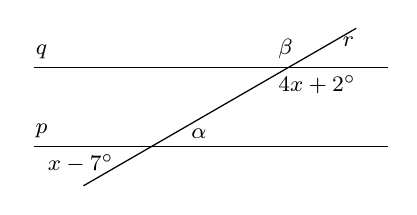
\begin{tikzpicture}
                        % \clip (0,0) rectangle (14.000000,10.000000);
                        {\footnotesize

                        % Drawing line Q
                        \draw [line width=0.016cm] (1.500000,1.500000) -- (6.000000,1.500000);%

                        % Drawing line P
                        \draw [line width=0.016cm] (1.500000,2.500000) -- (6.000000,2.500000);%

                        % Drawing line R
                        \draw [line width=0.016cm] (2.133975,1.000000) -- (5.598076,3.000000);%

                        % Marking point p
                        \draw (1.600000,1.500000) node [anchor=south] { $p$ };%

                        % Marking point q
                        \draw (1.600000,2.500000) node [anchor=south] { $q$ };%

                        % Marking point r
                        \draw (5.500000,3.000000) node [anchor=north] { $r$ };%

                        % Marking point \alpha
                        \draw (3.600000,1.500000) node [anchor=south] { $\alpha$ };%

                        % Marking point \beta
                        \draw (4.700000,2.500000) node [anchor=south] { $\beta$ };%

                        % Marking point {4x+2^\circ}
                        \draw (5.100000,2.500000) node [anchor=north] { ${4x+2^\circ}$ };%

                        % Marking point {x-7^\circ}
                        \draw (2.100000,1.500000) node [anchor=north] { ${x-7^\circ}$ };%
                        }
                    \end{tikzpicture} ~
                    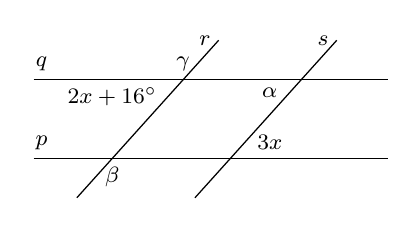
\begin{tikzpicture}
                        % \clip (0,0) rectangle (14.000000,10.000000);
                        {\footnotesize

                        % Drawing line Q
                        \draw [line width=0.016cm] (1.500000,1.500000) -- (6.000000,1.500000);%

                        % Drawing line P
                        \draw [line width=0.016cm] (1.500000,2.500000) -- (6.000000,2.500000);%

                        % Drawing line R
                        \draw [line width=0.016cm] (2.049798,1.000000) -- (3.850606,3.000000);%

                        % Drawing line S
                        \draw [line width=0.016cm] (3.549798,1.000000) -- (5.350606,3.000000);%

                        % Marking point p
                        \draw (1.600000,1.500000) node [anchor=south] { $p$ };%

                        % Marking point q
                        \draw (1.600000,2.500000) node [anchor=south] { $q$ };%

                        % Marking point r
                        \draw (3.500000,3.000000) node [anchor=west] { $r$ };%

                        % Marking point s
                        \draw (5.000000,3.000000) node [anchor=west] { $s$ };%

                        % Marking point \alpha
                        \draw (4.500000,2.500000) node [anchor=north] { $\alpha$ };%

                        % Marking point \beta
                        \draw (2.500000,1.500000) node [anchor=north] { $\beta$ };%

                        % Marking point \gamma
                        \draw (3.400000,2.500000) node [anchor=south] { $\gamma$ };%

                        % Marking point {3x}
                        \draw (4.500000,1.500000) node [anchor=south] { ${3x}$ };%

                        % Marking point {2x+16^\circ}
                        \draw (2.500000,2.500000) node [anchor=north] { ${2x+16^\circ}$ };%
                        }
                    \end{tikzpicture} ~
                    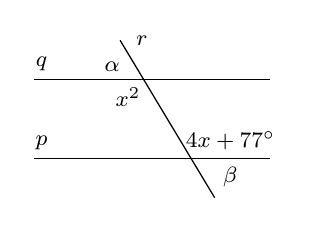
\begin{tikzpicture}
                        % \clip (0,0) rectangle (14.000000,10.000000);
                        {\footnotesize

                        % Drawing line Q
                        \draw [line width=0.016cm] (1.500000,1.500000) -- (4.500000,1.500000);%

                        % Drawing line P
                        \draw [line width=0.016cm] (1.500000,2.500000) -- (4.500000,2.500000);%

                        % Drawing line R
                        \draw [line width=0.016cm] (3.800430,1.000000) -- (2.598709,3.000000);%

                        % Marking point p
                        \draw (1.600000,1.500000) node [anchor=south] { $p$ };%

                        % Marking point q
                        \draw (1.600000,2.500000) node [anchor=south] { $q$ };%

                        % Marking point r
                        \draw (2.700000,3.000000) node [anchor=west] { $r$ };%

                        % Marking point \alpha
                        \draw (2.500000,2.500000) node [anchor=south] { $\alpha$ };%

                        % Marking point \beta
                        \draw (4.000000,1.500000) node [anchor=north] { $\beta$ };%

                        % Marking point {4x+77^\circ}
                        \draw (4.000000,1.500000) node [anchor=south] { ${4x+77^\circ}$ };%

                        % Marking point {x^2}
                        \draw (2.700000,2.500000) node [anchor=north] { ${x^2}$ };%
                        }
                    \end{tikzpicture}
                \end{figure}
            \end{naloga}
        

        
            \begin{naloga}
                Izračunajte velikosti vseh notranjih in zunanjih kotov trikotnika $\triangle ABC$, 
                če je vsota velikosti dveh zunanjih kotov $\alpha'+\gamma'=230^\circ$, vsota velikosti dveh notranjih kotov pa $\alpha+\beta=70^\circ$.
            \end{naloga}

            \begin{naloga}
                S skice preberite ustrezne podatke ter izračunajte velikosti kotov $\alpha$, $\beta$, $\gamma$ in $\delta$.
                Pri tem velja, da so premice $p$, $q$ in $r$ vzporedne.
                \begin{figure}
                    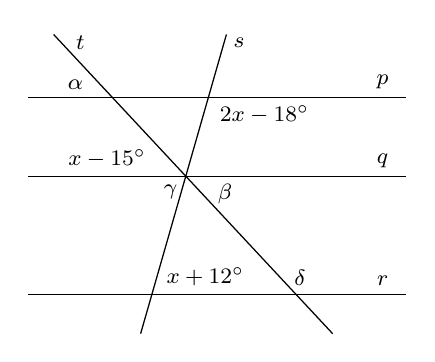
\begin{tikzpicture}
                        % \clip (0,0) rectangle (14.000000,10.000000);
                        {\footnotesize

                        % Drawing line Q
                        \draw [line width=0.016cm] (1.000000,3.000000) -- (5.800000,3.000000);%

                        % Drawing line P
                        \draw [line width=0.016cm] (1.000000,4.000000) -- (5.800000,4.000000);%

                        % Drawing line R
                        \draw [line width=0.016cm] (1.000000,1.500000) -- (5.800000,1.500000);%

                        % Drawing line S
                        \draw [line width=0.016cm] (2.426509,1.000000) -- (3.516142,4.800000);%

                        % Drawing line T
                        \draw [line width=0.016cm] (4.865030,1.000000) -- (1.321473,4.800000);%

                        % Marking point p
                        \draw (5.500000,4.000000) node [anchor=south] { $p$ };%

                        % Marking point q
                        \draw (5.500000,3.000000) node [anchor=south] { $q$ };%

                        % Marking point r
                        \draw (5.500000,1.500000) node [anchor=south] { $r$ };%

                        % Marking point s
                        \draw (3.500000,4.700000) node [anchor=west] { $s$ };%

                        % Marking point t
                        \draw (1.500000,4.700000) node [anchor=west] { $t$ };%

                        % Marking point \alpha
                        \draw (1.800000,4.000000) node [anchor=south east] { $\alpha$ };%

                        % Marking point \beta
                        \draw (3.300000,3.000000) node [anchor=north west] { $\beta$ };%

                        % Marking point \gamma
                        \draw (3.000000,3.000000) node [anchor=north east] { $\gamma$ };%

                        % Marking point \delta
                        \draw (4.450000,1.500000) node [anchor=south] { $\delta$ };%

                        % Marking point {x-15^\circ}
                        \draw (2.000000,3.000000) node [anchor=south] { ${x-15^\circ}$ };%

                        % Marking point {2x-18^\circ}
                        \draw (4.000000,4.000000) node [anchor=north] { ${2x-18^\circ}$ };%

                        % Marking point {x+12^\circ}
                        \draw (3.250000,1.500000) node [anchor=south] { ${x+12^\circ}$ };%
                        }
                    \end{tikzpicture}

                \end{figure}
            \end{naloga}

        

